%% bare_jrnl.tex
%% V1.4b
%% 2015/08/26
%% by Michael Shell
%% see http://www.michaelshell.org/
%% for current contact information.
%%
%% This is a skeleton file demonstrating the use of IEEEtran.cls
%% (requires IEEEtran.cls version 1.8b or later) with an IEEE
%% journal paper.
%%
%% Support sites:
%% http://www.michaelshell.org/tex/ieeetran/
%% http://www.ctan.org/pkg/ieeetran
%% and
%% http://www.ieee.org/

%%*************************************************************************
%% Legal Notice:
%% This code is offered as-is without any warranty either expressed or
%% implied; without even the implied warranty of MERCHANTABILITY or
%% FITNESS FOR A PARTICULAR PURPOSE! 
%% User assumes all risk.
%% In no event shall the IEEE or any contributor to this code be liable for
%% any damages or losses, including, but not limited to, incidental,
%% consequential, or any other damages, resulting from the use or misuse
%% of any information contained here.
%%
%% All comments are the opinions of their respective authors and are not
%% necessarily endorsed by the IEEE.
%%
%% This work is distributed under the LaTeX Project Public License (LPPL)
%% ( http://www.latex-project.org/ ) version 1.3, and may be freely used,
%% distributed and modified. A copy of the LPPL, version 1.3, is included
%% in the base LaTeX documentation of all distributions of LaTeX released
%% 2003/12/01 or later.
%% Retain all contribution notices and credits.
%% ** Modified files should be clearly indicated as such, including  **
%% ** renaming them and changing author support contact information. **
%%*************************************************************************


% *** Authors should verify (and, if needed, correct) their LaTeX system  ***
% *** with the testflow diagnostic prior to trusting their LaTeX platform ***
% *** with production work. The IEEE's font choices and paper sizes can   ***
% *** trigger bugs that do not appear when using other class files.       ***                          ***
% The testflow support page is at:
% http://www.michaelshell.org/tex/testflow/



\documentclass[journal]{IEEEtran}
%
% If IEEEtran.cls has not been installed into the LaTeX system files,
% manually specify the path to it like:
% \documentclass[journal]{../sty/IEEEtran}





% Some very useful LaTeX packages include:
% (uncomment the ones you want to load)


% *** MISC UTILITY PACKAGES ***
%
%\usepackage{ifpdf}
% Heiko Oberdiek's ifpdf.sty is very useful if you need conditional
% compilation based on whether the output is pdf or dvi.
% usage:
% \ifpdf
%   % pdf code
% \else
%   % dvi code
% \fi
% The latest version of ifpdf.sty can be obtained from:
% http://www.ctan.org/pkg/ifpdf
% Also, note that IEEEtran.cls V1.7 and later provides a builtin
% \ifCLASSINFOpdf conditional that works the same way.
% When switching from latex to pdflatex and vice-versa, the compiler may
% have to be run twice to clear warning/error messages.






% *** CITATION PACKAGES ***
%
%\usepackage{cite}
% cite.sty was written by Donald Arseneau
% V1.6 and later of IEEEtran pre-defines the format of the cite.sty package
% \cite{} output to follow that of the IEEE. Loading the cite package will
% result in citation numbers being automatically sorted and properly
% "compressed/ranged". e.g., [1], [9], [2], [7], [5], [6] without using
% cite.sty will become [1], [2], [5]--[7], [9] using cite.sty. cite.sty's
% \cite will automatically add leading space, if needed. Use cite.sty's
% noadjust option (cite.sty V3.8 and later) if you want to turn this off
% such as if a citation ever needs to be enclosed in parenthesis.
% cite.sty is already installed on most LaTeX systems. Be sure and use
% version 5.0 (2009-03-20) and later if using hyperref.sty.
% The latest version can be obtained at:
% http://www.ctan.org/pkg/cite
% The documentation is contained in the cite.sty file itself.






% *** GRAPHICS RELATED PACKAGES ***
%
\ifCLASSINFOpdf
  \usepackage[pdftex]{graphicx}
  % declare the path(s) where your graphic files are
  \graphicspath{{../pdf/}{../png/}}
  % and their extensions so you won't have to specify these with
  % every instance of \includegraphics
  \DeclareGraphicsExtensions{.pdf,.jpeg,.png}
\else
  % or other class option (dvipsone, dvipdf, if not using dvips). graphicx
  % will default to the driver specified in the system graphics.cfg if no
  % driver is specified.
  % \usepackage[dvips]{graphicx}
  % declare the path(s) where your graphic files are
  % \graphicspath{{../eps/}}
  % and their extensions so you won't have to specify these with
  % every instance of \includegraphics
  % \DeclareGraphicsExtensions{.eps}
\fi
% graphicx was written by David Carlisle and Sebastian Rahtz. It is
% required if you want graphics, photos, etc. graphicx.sty is already
% installed on most LaTeX systems. The latest version and documentation
% can be obtained at: 
% http://www.ctan.org/pkg/graphicx
% Another good source of documentation is "Using Imported Graphics in
% LaTeX2e" by Keith Reckdahl which can be found at:
% http://www.ctan.org/pkg/epslatex
%
% latex, and pdflatex in dvi mode, support graphics in encapsulated
% postscript (.eps) format. pdflatex in pdf mode supports graphics
% in .pdf, .jpeg, .png and .mps (metapost) formats. Users should ensure
% that all non-photo figures use a vector format (.eps, .pdf, .mps) and
% not a bitmapped formats (.jpeg, .png). The IEEE frowns on bitmapped formats
% which can result in "jaggedy"/blurry rendering of lines and letters as
% well as large increases in file sizes.
%
% You can find documentation about the pdfTeX application at:
% http://www.tug.org/applications/pdftex



\usepackage{multirow}

% *** MATH PACKAGES ***
%
\usepackage{amsmath}
\usepackage{amssymb}
\usepackage{subcaption}
% A popular package from the American Mathematical Society that provides
% many useful and powerful commands for dealing with mathematics.
%
% Note that the amsmath package sets \interdisplaylinepenalty to 10000
% thus preventing page breaks from occurring within multiline equations. Use:
%\interdisplaylinepenalty=2500
% after loading amsmath to restore such page breaks as IEEEtran.cls normally
% does. amsmath.sty is already installed on most LaTeX systems. The latest
% version and documentation can be obtained at:
% http://www.ctan.org/pkg/amsmath





% *** SPECIALIZED LIST PACKAGES ***
%
%\usepackage{algorithmic}
% algorithmic.sty was written by Peter Williams and Rogerio Brito.
% This package provides an algorithmic environment fo describing algorithms.
% You can use the algorithmic environment in-text or within a figure
% environment to provide for a floating algorithm. Do NOT use the algorithm
% floating environment provided by algorithm.sty (by the same authors) or
% algorithm2e.sty (by Christophe Fiorio) as the IEEE does not use dedicated
% algorithm float types and packages that provide these will not provide
% correct IEEE style captions. The latest version and documentation of
% algorithmic.sty can be obtained at:
% http://www.ctan.org/pkg/algorithms
% Also of interest may be the (relatively newer and more customizable)
% algorithmicx.sty package by Szasz Janos:
% http://www.ctan.org/pkg/algorithmicx




% *** ALIGNMENT PACKAGES ***
%
%\usepackage{array}
% Frank Mittelbach's and David Carlisle's array.sty patches and improves
% the standard LaTeX2e array and tabular environments to provide better
% appearance and additional user controls. As the default LaTeX2e table
% generation code is lacking to the point of almost being broken with
% respect to the quality of the end results, all users are strongly
% advised to use an enhanced (at the very least that provided by array.sty)
% set of table tools. array.sty is already installed on most systems. The
% latest version and documentation can be obtained at:
% http://www.ctan.org/pkg/array


% IEEEtran contains the IEEEeqnarray family of commands that can be used to
% generate multiline equations as well as matrices, tables, etc., of high
% quality.




% *** SUBFIGURE PACKAGES ***
%\ifCLASSOPTIONcompsoc
%  \usepackage[caption=false,font=normalsize,labelfont=sf,textfont=sf]{subfig}
%\else
%  \usepackage[caption=false,font=footnotesize]{subfig}
%\fi
% subfig.sty, written by Steven Douglas Cochran, is the modern replacement
% for subfigure.sty, the latter of which is no longer maintained and is
% incompatible with some LaTeX packages including fixltx2e. However,
% subfig.sty requires and automatically loads Axel Sommerfeldt's caption.sty
% which will override IEEEtran.cls' handling of captions and this will result
% in non-IEEE style figure/table captions. To prevent this problem, be sure
% and invoke subfig.sty's "caption=false" package option (available since
% subfig.sty version 1.3, 2005/06/28) as this is will preserve IEEEtran.cls
% handling of captions.
% Note that the Computer Society format requires a larger sans serif font
% than the serif footnote size font used in traditional IEEE formatting
% and thus the need to invoke different subfig.sty package options depending
% on whether compsoc mode has been enabled.
%
% The latest version and documentation of subfig.sty can be obtained at:
% http://www.ctan.org/pkg/subfig




% *** FLOAT PACKAGES ***
%
%\usepackage{fixltx2e}
% fixltx2e, the successor to the earlier fix2col.sty, was written by
% Frank Mittelbach and David Carlisle. This package corrects a few problems
% in the LaTeX2e kernel, the most notable of which is that in current
% LaTeX2e releases, the ordering of single and double column floats is not
% guaranteed to be preserved. Thus, an unpatched LaTeX2e can allow a
% single column figure to be placed prior to an earlier double column
% figure.
% Be aware that LaTeX2e kernels dated 2015 and later have fixltx2e.sty's
% corrections already built into the system in which case a warning will
% be issued if an attempt is made to load fixltx2e.sty as it is no longer
% needed.
% The latest version and documentation can be found at:
% http://www.ctan.org/pkg/fixltx2e


%\usepackage{stfloats}
% stfloats.sty was written by Sigitas Tolusis. This package gives LaTeX2e
% the ability to do double column floats at the bottom of the page as well
% as the top. (e.g., "\begin{figure*}[!b]" is not normally possible in
% LaTeX2e). It also provides a command:
%\fnbelowfloat
% to enable the placement of footnotes below bottom floats (the standard
% LaTeX2e kernel puts them above bottom floats). This is an invasive package
% which rewrites many portions of the LaTeX2e float routines. It may not work
% with other packages that modify the LaTeX2e float routines. The latest
% version and documentation can be obtained at:
% http://www.ctan.org/pkg/stfloats
% Do not use the stfloats baselinefloat ability as the IEEE does not allow
% \baselineskip to stretch. Authors submitting work to the IEEE should note
% that the IEEE rarely uses double column equations and that authors should try
% to avoid such use. Do not be tempted to use the cuted.sty or midfloat.sty
% packages (also by Sigitas Tolusis) as the IEEE does not format its papers in
% such ways.
% Do not attempt to use stfloats with fixltx2e as they are incompatible.
% Instead, use Morten Hogholm'a dblfloatfix which combines the features
% of both fixltx2e and stfloats:
%
% \usepackage{dblfloatfix}
% The latest version can be found at:
% http://www.ctan.org/pkg/dblfloatfix




%\ifCLASSOPTIONcaptionsoff
%  \usepackage[nomarkers]{endfloat}
% \let\MYoriglatexcaption\caption
% \renewcommand{\caption}[2][\relax]{\MYoriglatexcaption[#2]{#2}}
%\fi
% endfloat.sty was written by James Darrell McCauley, Jeff Goldberg and 
% Axel Sommerfeldt. This package may be useful when used in conjunction with 
% IEEEtran.cls'  captionsoff option. Some IEEE journals/societies require that
% submissions have lists of figures/tables at the end of the paper and that
% figures/tables without any captions are placed on a page by themselves at
% the end of the document. If needed, the draftcls IEEEtran class option or
% \CLASSINPUTbaselinestretch interface can be used to increase the line
% spacing as well. Be sure and use the nomarkers option of endfloat to
% prevent endfloat from "marking" where the figures would have been placed
% in the text. The two hack lines of code above are a slight modification of
% that suggested by in the endfloat docs (section 8.4.1) to ensure that
% the full captions always appear in the list of figures/tables - even if
% the user used the short optional argument of \caption[]{}.
% IEEE papers do not typically make use of \caption[]'s optional argument,
% so this should not be an issue. A similar trick can be used to disable
% captions of packages such as subfig.sty that lack options to turn off
% the subcaptions:
% For subfig.sty:
\let\MYorigsubfloat\subfloat
\renewcommand{\subfloat}[2][\relax]{\MYorigsubfloat[]{#2}}
% However, the above trick will not work if both optional arguments of
% the \subfloat command are used. Furthermore, there needs to be a
% description of each subfigure *somewhere* and endfloat does not add
% subfigure captions to its list of figures. Thus, the best approach is to
% avoid the use of subfigure captions (many IEEE journals avoid them anyway)
% and instead reference/explain all the subfigures within the main caption.
% The latest version of endfloat.sty and its documentation can obtained at:
% http://www.ctan.org/pkg/endfloat
%
% The IEEEtran \ifCLASSOPTIONcaptionsoff conditional can also be used
% later in the document, say, to conditionally put the References on a 
% page by themselves.




% *** PDF, URL AND HYPERLINK PACKAGES ***
%
%\usepackage{url}
% url.sty was written by Donald Arseneau. It provides better support for
% handling and breaking URLs. url.sty is already installed on most LaTeX
% systems. The latest version and documentation can be obtained at:
% http://www.ctan.org/pkg/url
% Basically, \url{my_url_here}.




% *** Do not adjust lengths that control margins, column widths, etc. ***
% *** Do not use packages that alter fonts (such as pslatex).         ***
% There should be no need to do such things with IEEEtran.cls V1.6 and later.
% (Unless specifically asked to do so by the journal or conference you plan
% to submit to, of course. )


% correct bad hyphenation here
\hyphenation{op-tical net-works semi-conduc-tor}


\begin{document}
%
% paper title
% Titles are generally capitalized except for words such as a, an, and, as,
% at, but, by, for, in, nor, of, on, or, the, to and up, which are usually
% not capitalized unless they are the first or last word of the title.
% Linebreaks \\ can be used within to get better formatting as desired.
% Do not put math or special symbols in the title.
\title{Comparative Analysis of Deep Neural Network Models for Time Series Classification}
%
%
% author names and IEEE memberships
% note positions of commas and nonbreaking spaces ( ~ ) LaTeX will not break
% a structure at a ~ so this keeps an author's name from being broken across
% two lines.
% use \thanks{} to gain access to the first footnote area
% a separate \thanks must be used for each paragraph as LaTeX2e's \thanks
% was not built to handle multiple paragraphs
%

\author{Kieran Molloy, 35762970}

% note the % following the last \IEEEmembership and also \thanks - 
% these prevent an unwanted space from occurring between the last author name
% and the end of the author line. i.e., if you had this:
% 
% \author{....lastname \thanks{...} \thanks{...} }
%                     ^------------^------------^----Do not want these spaces!
%
% a space would be appended to the last name and could cause every name on that
% line to be shifted left slightly. This is one of those "LaTeX things". For
% instance, "\textbf{A} \textbf{B}" will typeset as "A B" not "AB". To get
% "AB" then you have to do: "\textbf{A}\textbf{B}"
% \thanks is no different in this regard, so shield the last } of each \thanks
% that ends a line with a % and do not let a space in before the next \thanks.
% Spaces after \IEEEmembership other than the last one are OK (and needed) as
% you are supposed to have spaces between the names. For what it is worth,
% this is a minor point as most people would not even notice if the said evil
% space somehow managed to creep in.



% The paper headers
\markboth{SCC413 Computer Vision Coursework 1 - Kieran Molloy}%
{SCC413 Computer Vision Coursework 1 - Kieran Molloy}
% The only time the second header will appear is for the odd numbered pages
% after the title page when using the twoside option.
% 
% *** Note that you probably will NOT want to include the author's ***
% *** name in the headers of peer review papers.                   ***
% You can use \ifCLASSOPTIONpeerreview for conditional compilation here if
% you desire.




% If you want to put a publisher's ID mark on the page you can do it like
% this:
%\IEEEpubid{0000--0000/00\$00.00~\copyright~2015 IEEE}
% Remember, if you use this you must call \IEEEpubidadjcol in the second
% column for its text to clear the IEEEpubid mark.



% use for special paper notices
%\IEEEspecialpapernotice{(Invited Paper)}




% make the title area
\maketitle

% As a general rule, do not put math, special symbols or citations
% in the abstract or keywords.
\begin{abstract}
The implementation of automatic Electrocargiogram (ECG) classification poses massive real world benefits, allowing a more streamlined patient diagnosis pathway for heart conditions that would not be found without cardiologist input. ECG Classification is a complex time series problem, and there are many machine learning solutions that can be used to analyse and classify ECG data - these are mostly hand-crated heuristics or feature selected. This paper poses five deep learning time series classification architectures that can classify ECG data swiftly and with increased performance than an average cardiologist, furthermore using Wilcoxon-Holm post-hoc analysis to determine if a set of classifers are statistically significantly different.
\end{abstract}

% Note that keywords are not normally used for peerreview papers.
\begin{IEEEkeywords}
DNN, CNN, TSC, MLP, RESNET, RNN, MCNN, LENET
\end{IEEEkeywords}






% For peer review papers, you can put extra information on the cover
% page as needed:
% \ifCLASSOPTIONpeerreview
% \begin{center} \bfseries EDICS Category: 3-BBND \end{center}
% \fi
%
% For peerreview papers, this IEEEtran command inserts a page break and
% creates the second title. It will be ignored for other modes.
\IEEEpeerreviewmaketitle



\section{Introduction}
% The very first letter is a 2 line initial drop letter followed
% by the rest of the first word in caps.
% 
% form to use if the first word consists of a single letter:
% \IEEEPARstart{A}{demo} file is ....
% 
% form to use if you need the single drop letter followed by
% normal text (unknown if ever used by the IEEE):
% \IEEEPARstart{A}{}demo file is ....
% 
% Some journals put the first two words in caps:
% \IEEEPARstart{T}{his demo} file is ....
% 
% Here we have the typical use of a "T" for an initial drop letter
% and "HIS" in caps to complete the first word.
\IEEEPARstart{W}{ithin} the previous ten years Deep Learning has made significant strides and Time Series Classification poses one of the largest challenges. With temporal data becoming widely available, there has been a significant increase of algorithms proposed recently \cite{IsmailFawaz2018deep}. With temporal data requiring the order to be maintained, the time series classification problem is encountered in many scenarios, such as ECG - as is the main focus within this report, acoustic classification and cyber-security. Most general heart problems can be diagnosed from ECG signals, and with hundreds of millions of these recorded annually, physicians are not able to manually review and diagnose conditions. This motivates the use of Machine Learning approaches to swiftly and accurately diagnose these heart irregularities for further review by a physician. The main disadvantages of machine learning approaches is the inability to find the most appropriate features that give high classification accuracy. Deep Learning architectures can resolve this problem with this paper focusing on the end-to-end deep learning models, and implementing a series of models on selected ECG datasets. The results are investigated using Critical difference diagrams - leveraging Wilcoxon and Friedmann tests, and evaluating classification metrics. 

\section{Background}
ECG Classification is a difficult problem, and has had significant attention from the medical community and increasingly computer scientists that specialise in machine learning approaches. Recently a 34-layer convolutional neural network was capable of exceeding the average cardiologists performance in precision and recall \cite{rajpurkar2017}. Other works present binary ECG classification algorithms that use manual heuristics or feature engineering, these work well in single scenarios but cannot be transitioned to solve other ECG classification problems, therefore it is of interest to define a general model for ECG classification that is able to be translated to all ECG problems. The ECG data which can be obtained from patients is time series data, often a duration of around 45 seconds and a sampling time of 0.03s. As stated in the introduction it is desireable to remove the feature selection aspect of these classification algorithms, as that requires expert and subject specific knowledge. Therefore this paper will discover what deep learning approaches have been succesful for other time series classification problems and translate those architectures to the ECG classification problem.

Deep learning approaches for Time Series Classification (TSC) are separated into two key groups \cite{langkvist2014}; 
\begin{itemize}
    \item generative
    \item discriminative
\end{itemize}
These are further separated into sub-groups, shown in Figure \ref{fig:dl-groups}

\subsection{Generative Models}
Generative models often have an unsupervised training step that precedes the learning phase of the classifier \cite{langkvist2014}. This type of network is known as a model-based classifier \cite{Bagnall2016b}. Some of these approaches include auto-regressive models \cite{bagnall2014}, hidden markov models \cite{kotsifakos2014} and kernel models \cite{chen2013}. The goal for generative models is to create/find a representation of time series prior to training a classifier \cite{IsmailFawaz2018deep}, \cite{langkvist2014}, , usually to model a time series, classifiers are preceded by an unsupervised pre-training phase such as stacked denoising auto-encoders (SDAEs) \cite{bengio2013}, \cite{hu2016}. A generative CNN-based model was proposed in \cite{wang2016}; \cite{mittelman2015} where the authors introduced a deconvolutional operation followed by an upsampling technique that helps in reconstructing a multivariate time series. Deep Belief Networks (DBNs) were also used to model the latent features in an unsupervised manner which are then leverages to classify univariate and multivariate time series \cite{wang2017a}, \cite{banerjee2017}. In \cite{mehdiyev2017}, \cite{malhotra2017}, \cite{rajan2018}, an RNN auto-encoder was designed to first generate the time series then using the learned latent representation, they trained a classifier (such as SVM or Random Forest ensemble method) on top of these representations to predict the class of a given input time series.
Other studies such as \cite{aswolinskiy2017}, \cite{bianchi2020}, \cite{chouikhi2018}, \cite{ma2016} used self-predict modelling for time series classification where Echo State Networks were first used to re-construct the time series and then the learned representation in the reservoir space was utilised for classification, they have been used to define a kernel over the learned representation followed by an SVM or MLP classifier \cite{chen2013}, \cite{chen2015}, \cite{che2017}. Other papers have presented a meta-learning evolutionary-based algorithm to construct optimal architecture for univariate or multivariate time series \cite{wang2016}, \cite{gong2019}. 

\begin{figure}[h]
    \centering
    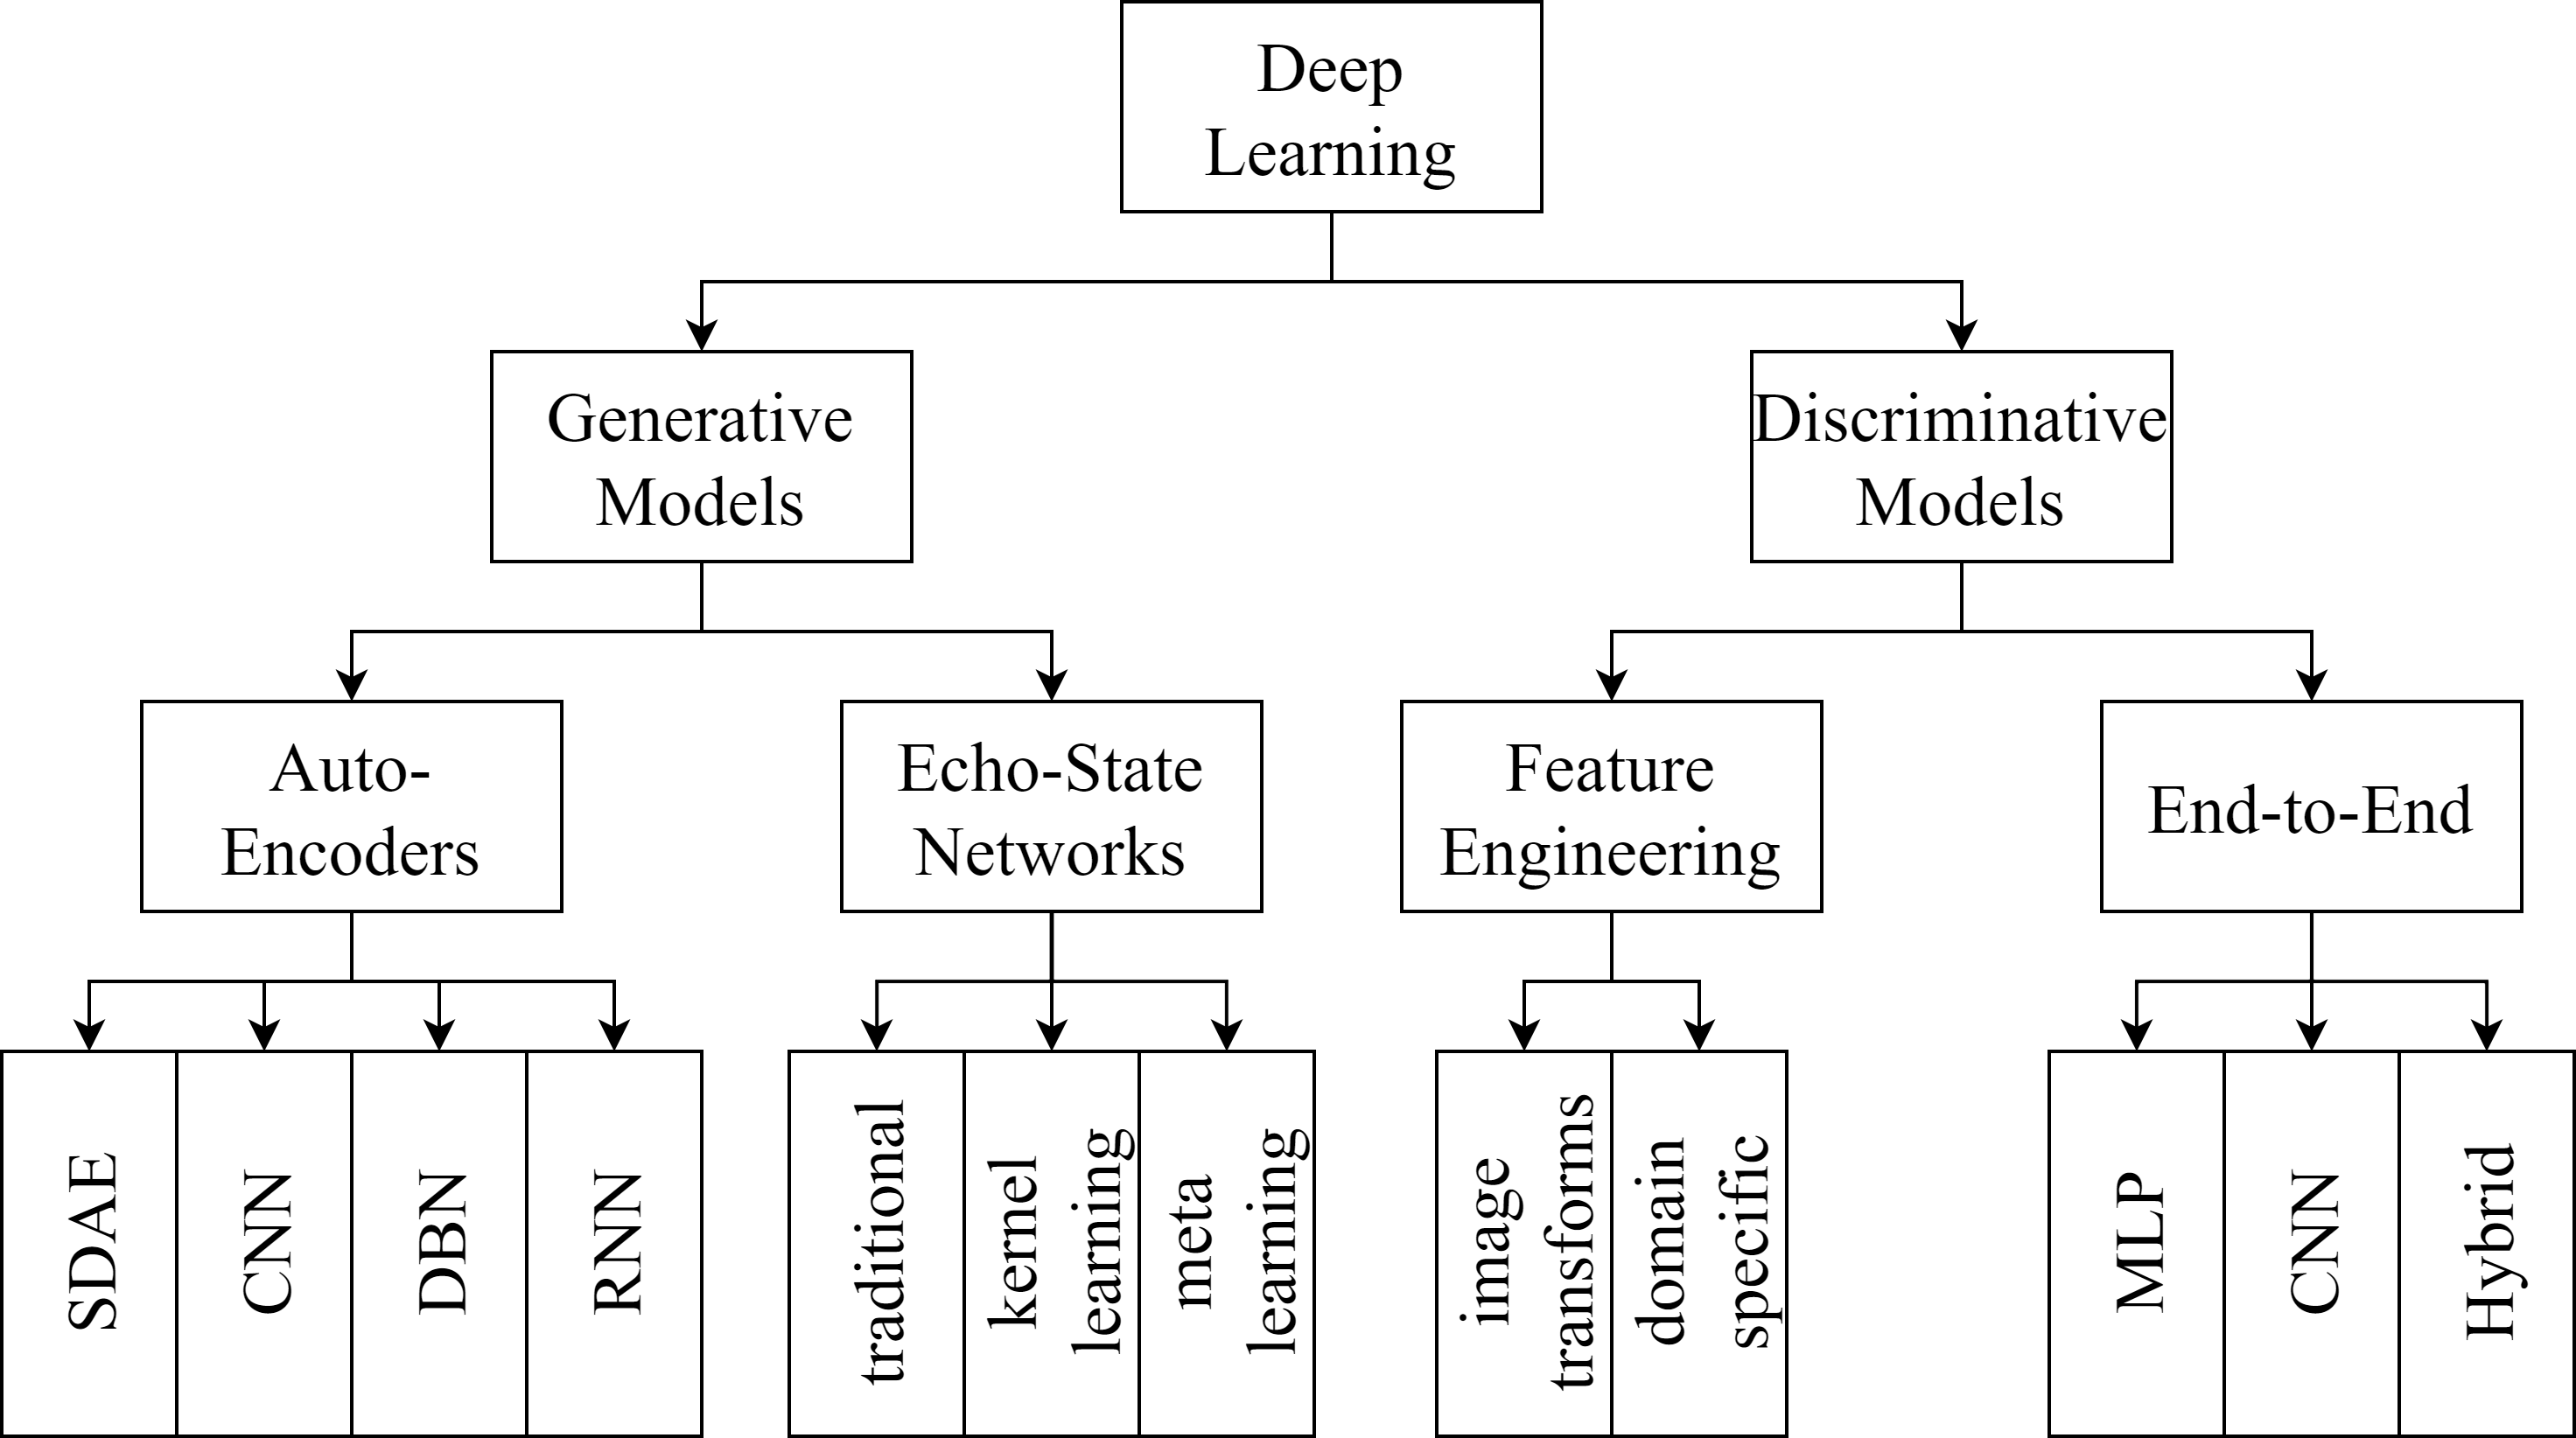
\includegraphics[width=3.5in]{assets/DL_approaches.png}
    
    \caption{Hierarchy of deep learning approaches for time series classification from  \cite{IsmailFawaz2018deep}\cite{langkvist2014}}
    \label{fig:dl-groups}
\end{figure}

\subsection{Discriminative Models}
A discriminative deep learning model is a classifier, or regressor, that directly learns the mapping between an input time series and outputs a probability distribution over the class variables in a dataset. The most frequently applied feature extraction method for 

\section{Methodologies}

Formally, A univariate time series $X = \{x_1, x_2, \dots, x_T\}$ is an ordered set of real values, where the length of $X$ is equal to the number of real values $T$. Naturally, an $M$-dimensional time series, MTS, can be defined as $\bar{X} = [X^1, X^2, \dots, X^T]$ which consists of $M$ different univariate time series where $X_i \in \mathbb{R}^T$.

A deep neural network is a composition of parametric functions, known as layers, where each function is a representation of the input domain \cite{papernot2018}. Each layer $l_i$ contains any integer number of neurons, which are independent compute units that return the layer output, traditionally these also apply a non-linearity function such as relu or sigmoid. These layers are chained where layer $l_i$ takes input from layer $l_{i-1}$ and returns its output to layer $l_{i+1}$, these transformations are controlled by $\theta_i$, otherwise known as weights, which link the layers together. Hence, given an input dataset $x$, a neural network can be defined as
\begin{equation}\label{eq:dnn}
    f_L(\theta_L, x) = f_{L-1}(\theta_{L-1}, f_{L-2}(\theta_{L-2}, \dots, f_1(\theta_1, x)))
\end{equation}
where $f_i$ is the non-linearity function for layer $i$. This process is known as feed-forward propagation.



\subsection{Multi-Layer Perceptron}
A Multi-Layer Perceptron (MLP) constitutes the simplest form of a deep learning model, the architecture of the model is known as fully connected - since the neurons in layer $l_i$ are connected to every neuron in layer $l_{i-1}$ where there are $i \in [1,L]$ layers, each of these connections hold a weight. A general form of an MLP applied to a time series $X$

\begin{equation}\label{eq:mlp}
A_{l_i} = f(w_{l_i} \cdot X + b)
\end{equation}

with $w_{l_i}$ being the set of weights, $b$ the bias term and $A_{l_i}$ the activation function of the neurons in layer $l_i$. A problem with MLP's is the inability to exhibit any spatial invariance, so temporal information is lost and each element is considered independently. The final layer takes the form of a probabilistic distribution over the class variables, often a softmax or sigmoid, and has equal neurons to the number of classes in the dataset. The weights presented in equation \ref{eq:mlp} are learned automatically using an optimisation algorithm that minimises an objective function - generally the Adam optimiser is used throughout this paper. For an optimiser to approximate the error of values, a loss function that can quantify this error needs to be defined, a commonly used loss function is categorical cross entropy:
\begin{equation}\label{eq:catcrossentropy}
    L(X) = - \sum_{j=1}^{K}{Y_j \log \hat{Y}_j}
\end{equation}
where $L$ is the loss of time series $X$. Naturally, the average loss of the whole training set is defined by:
\begin{equation}\label{eq:model-loss}
    J(W) = \frac{1}{N} \sum_{n=1}^{N}{L(X_n)}.
\end{equation}
Hence, the loss function minimises the learned weights $w$ using a gradient descent method:
\begin{equation}
    w = w - \alpha \frac{\partial J}{\partial w} \bigg\rvert \ \forall \ w \in W
\end{equation}
where $\alpha$ is the learning rate of the optimisation algorithm. This model is capable of auto-tuning the parameters $w$ in order to search and find a local minimum $J$. The partial derivative cannot be directly computed with respect to a certain parameter $w$, the chain rule of derivative is employed which is in fact the main idea behind the backpropagation algorithm \cite{lecun1998b}.

\subsection{Convolutional Neural Networks}
The idea of using artificial neural networks for processing images was proposed in \cite{lecun1998a} which automated the recognition of numbers, leading to the development of the widely used MNIST dataset today, this paper proposed an architecture now known as Convolutional Neural Networks (CNN). A CNN consists of input and outputs layers, as well as hidden layers, like the MLP described previously. The hidden layers consist of convolutional layer, pooling layer and a fully connected classifier - which is a perceptron based upon the features obtained on previous layers. 
% Defining an image, $I$, of dimension $m \times n \times p$, where $m$ is the rows, $n$ is the columns, $p$ is the colour depth,  is the input of the CNN. Images that are RGB have a colour depth of 3, whereas HDMI 2.1 has support for up to 48 bits \cite{hdmi2.1}, but around 24 bits is more common for devices to use. The CNN input can be described as three dimensional function $I(x, y, z)$, where $0 \leq x < m$, $0 \leq y < n$ and $0 \leq z < D$ are the spatial coordinates, with the amplitude $I$ at any point $(x, y, z)$ is the intensity of pixels at that point, and obtaining characteristics in convolutional layers can be represented as:
% \begin{equation}\label{eq:cnn-images}
%     I_f(x,y) = b + \sum_{i=-t}^{t}\sum_{j=-t}^{t}\sum_{k=0}^{p-1}{W_{i,j,k} \cdot I(x+i, y+j, k)}
% \end{equation}
% where $I_f$ is the feature map, $W_{i,j,k}$ is the filter for processing $p$ two-dimensional arrays, $b$ is the offset / bias and $t = \frac{w-1}{2}$. CNN uses a larger number of filters in the convolutional layer, which leads to a sharp increase in the amount of data that needs to be processed in the network and so the pooling layer is used to reduce them. Figure \ref{fig:cnn-pooling} schematically shows a max pooling operation using a filter mask of size $w x w$ and stride $w$. The output of this layer is transmitted to the input of the classifier which is organised a traditional MLP.

\begin{figure}[!t]
    \centering
    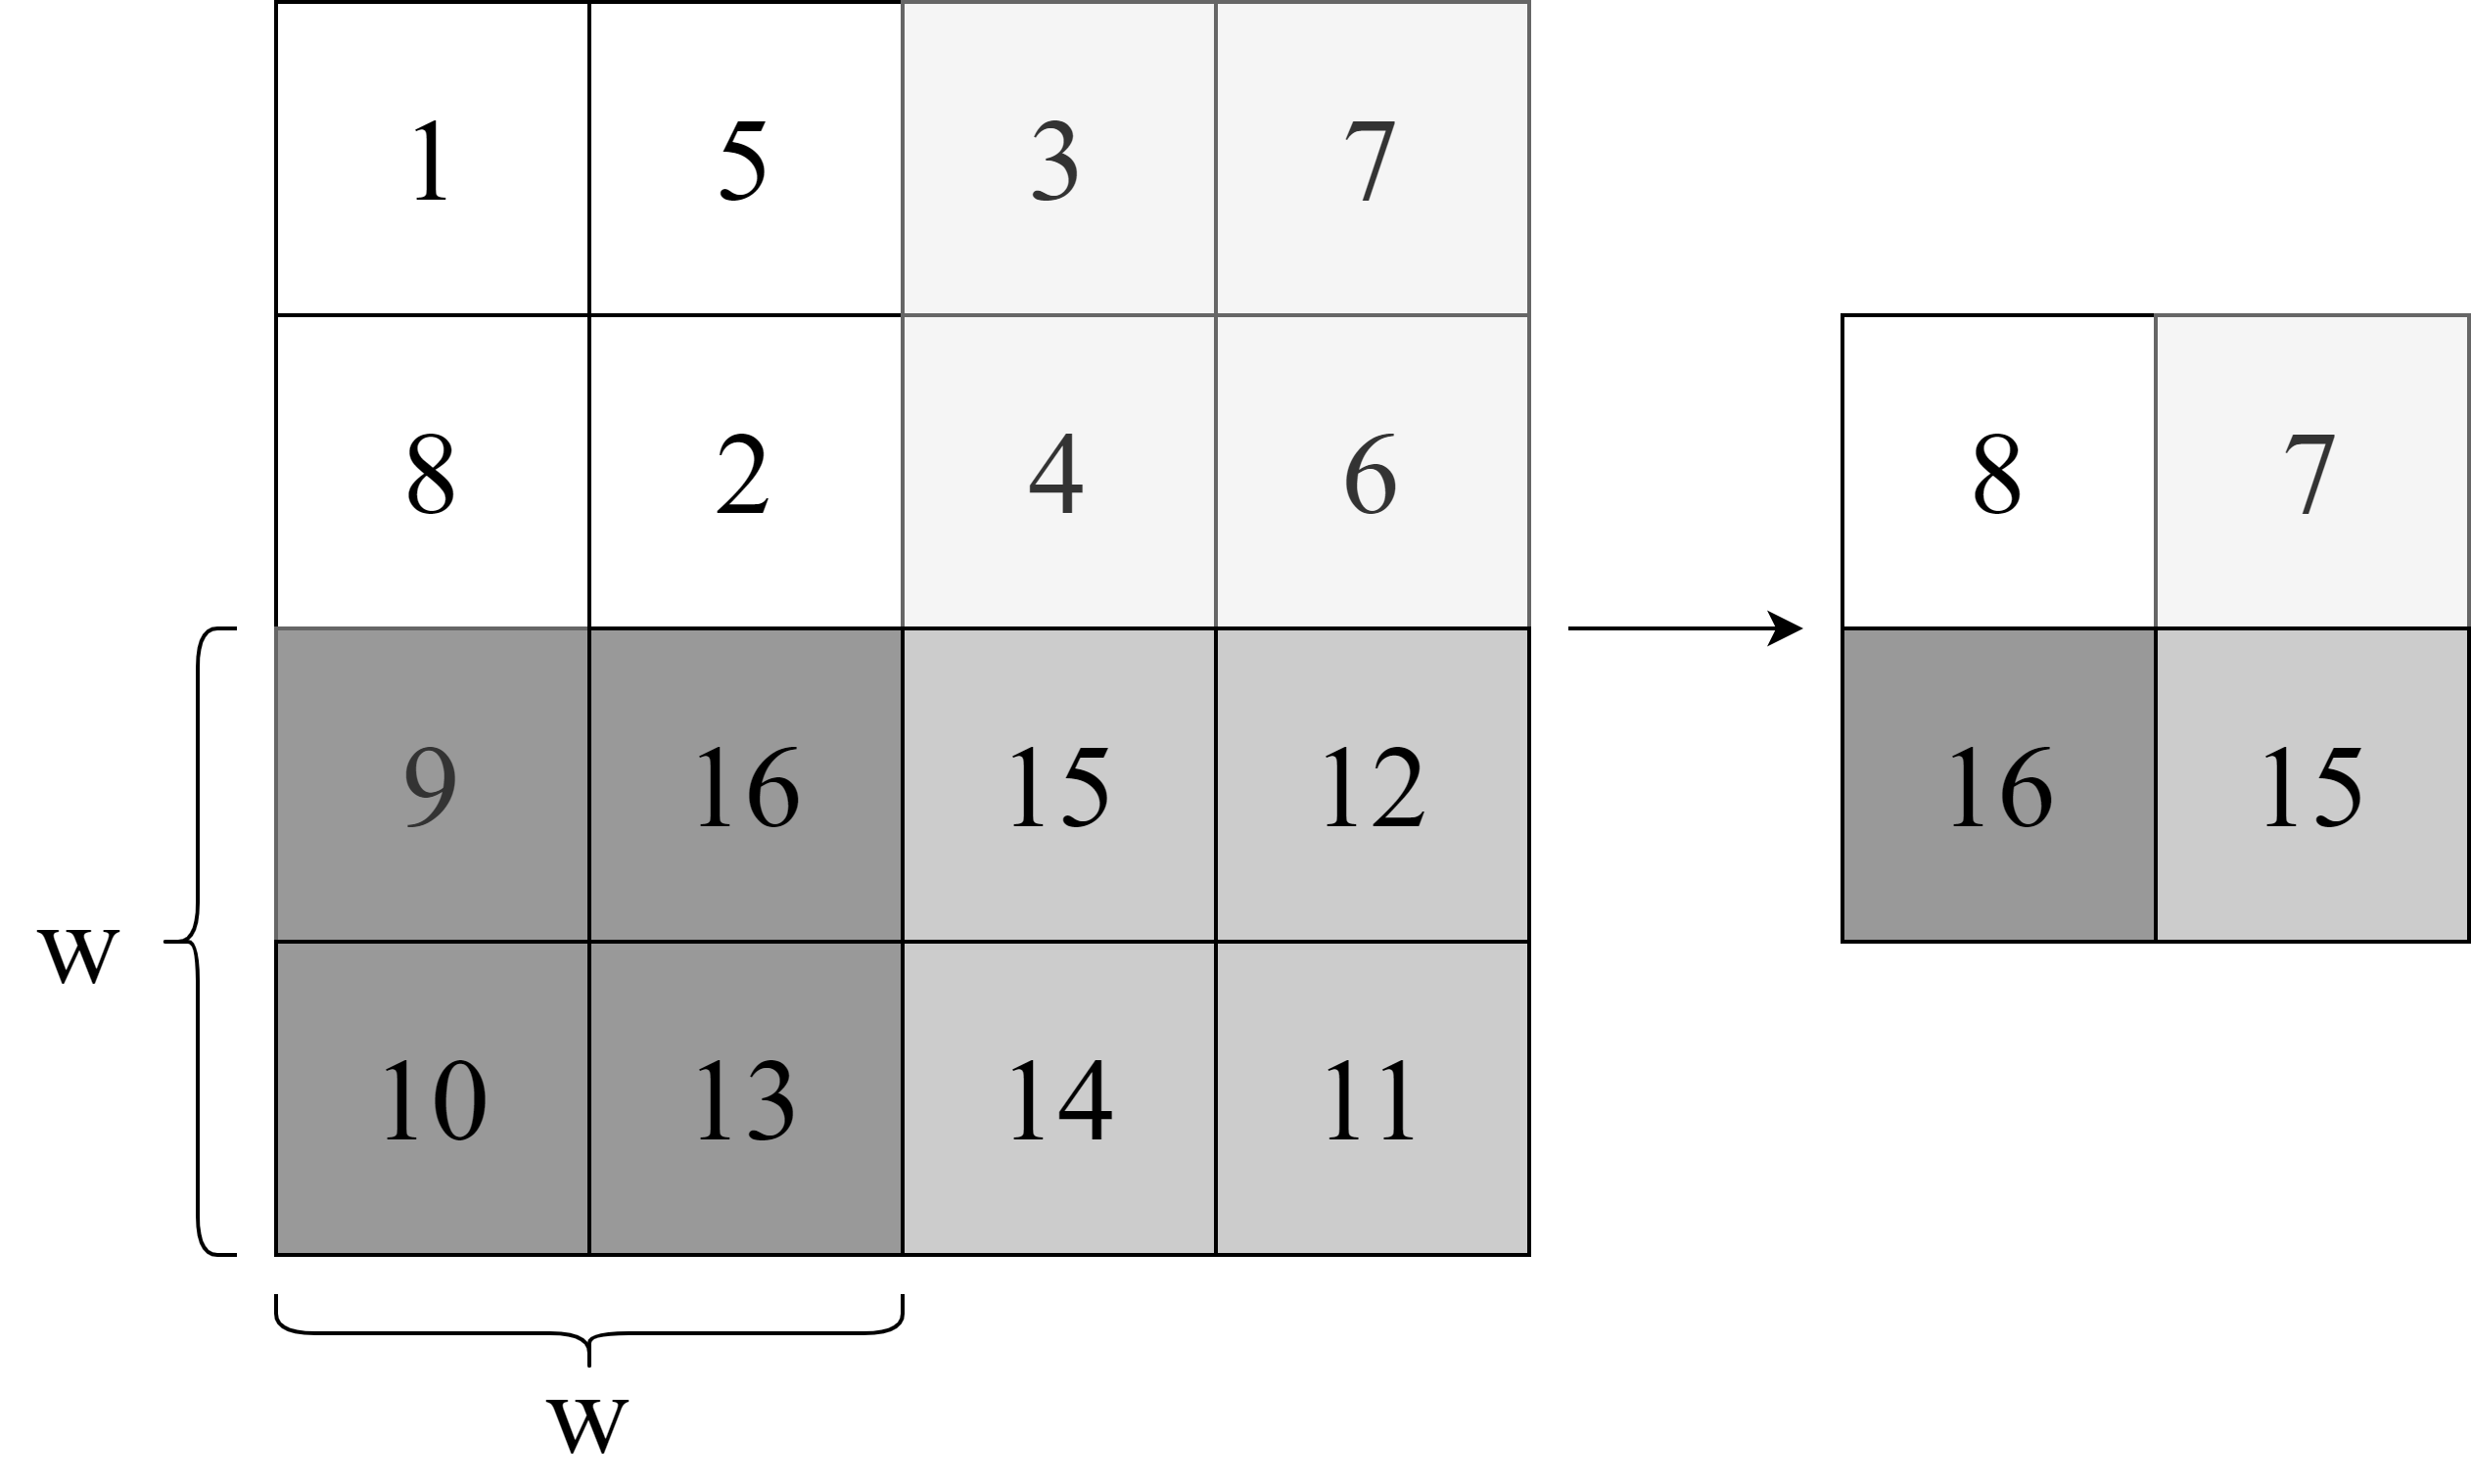
\includegraphics[width=2.5in]{assets/CNN_pooling_layer.png}
    
    \caption{The principle of operation of the pooling layer that implements the max pooling operation on a 2-dimensional array}
    \label{fig:cnn-pooling}
    
\end{figure}

% Applying this concept for images, 2-dimensional arrays, to time series analysis \cite{gamboa2017}. 
A convolution can be seen as applying a sliding filter over a time series. Unlike the 2-dimensional variant which have width and height, the filters exhibit a single dimension only which represents time. The filter is synonymous with a generic non-linear transformation of the time series - if the time series is convoluted with a filter of size 3 with a univariate time series, by setting the filter to $[\frac{1}{3}, \frac{1}{3}, \frac{1}{3}]$, the convolution will result in applying a moving average with a sliding window of length 3. A general form of this for any centered time step $t$:
\begin{equation}\label{eq:cnn}
    C_t = f(w \cdot X_{t-\frac{l}{2}, t+\frac{l}{2}} + b) \ \big\rvert \ \forall \ t \in [1, T]
\end{equation}
where $C$ is the convolution, the dot product of time series $X$ and filter $w$ with lengths $T$ and $l$ respectively, the bias parameter $b$ and a non-linear function $f$ such as ReLU. Applying several filters on a time series will result in a multivariate time series whose dimensions are equal to the number of filters used. An intuition behind applying several filters on an input time series would be to learn multiple discriminative features useful for the classification task. Unlike the previously discussed MLP's, the same convolution will be used to find the result for all time stamps $t$. This is known as weight sharting and is a powerful property of the CNN's which enable filter learning with no invariance across time. When considering a multi-variate time series as input to a convolutional layer, the filter is adapted to have dimensions equal the the time series instead of the ordinary single dimension, $t$, time.
Weights are learned automatically, since they highly depend in the targeted dataset and its attributes, the optimal filter is custom to these, where optimal is a filter that enables the classifier to easily discrimate between the classes - generally, when applied, this takes the form of a pooling operation, followed by a discriminative filter, followed by the classifier.
Local Pooling, such as average or max, with max pooling demonstrated in Figure \ref{fig:cnn-pooling}, takes an input time series and reduces it length $T$ by aggregating over a sliding window of the time series. For example, if the sliding windows length is 4, the resulting pooled time series with have length $\frac{T}{4}$ (where $T \mod 4 = 0$ ). In addition to pooling, some architectures include layers that normalise to increase convergence speed, for time series data, the batch normalisation operation is performed over each channel, thus preventing a covariate shift across a batch of time series \cite{ioffe2015}. An alternative approach, similar to z-normalisation, is to normalise each instance instead of batch, learning the mean and standard deviation of each instance for each layer via gradient descent \cite{ulyanov2016}.
The final discriminative layer takes the result of the convolutions and returns a probability distribution over the classes, this layer is usually a softmax operation. In order to train the network, and learn the parameters, the process is the same as the MLP described above, a forward pass, followed by back-propagation \cite{lecun1998b}. An example of a CNN architecture for time series classification with three convolutional layers is illustrated in Figure \ref{fig:cnn-layers}.

\begin{figure*}[!t]
    \centering
    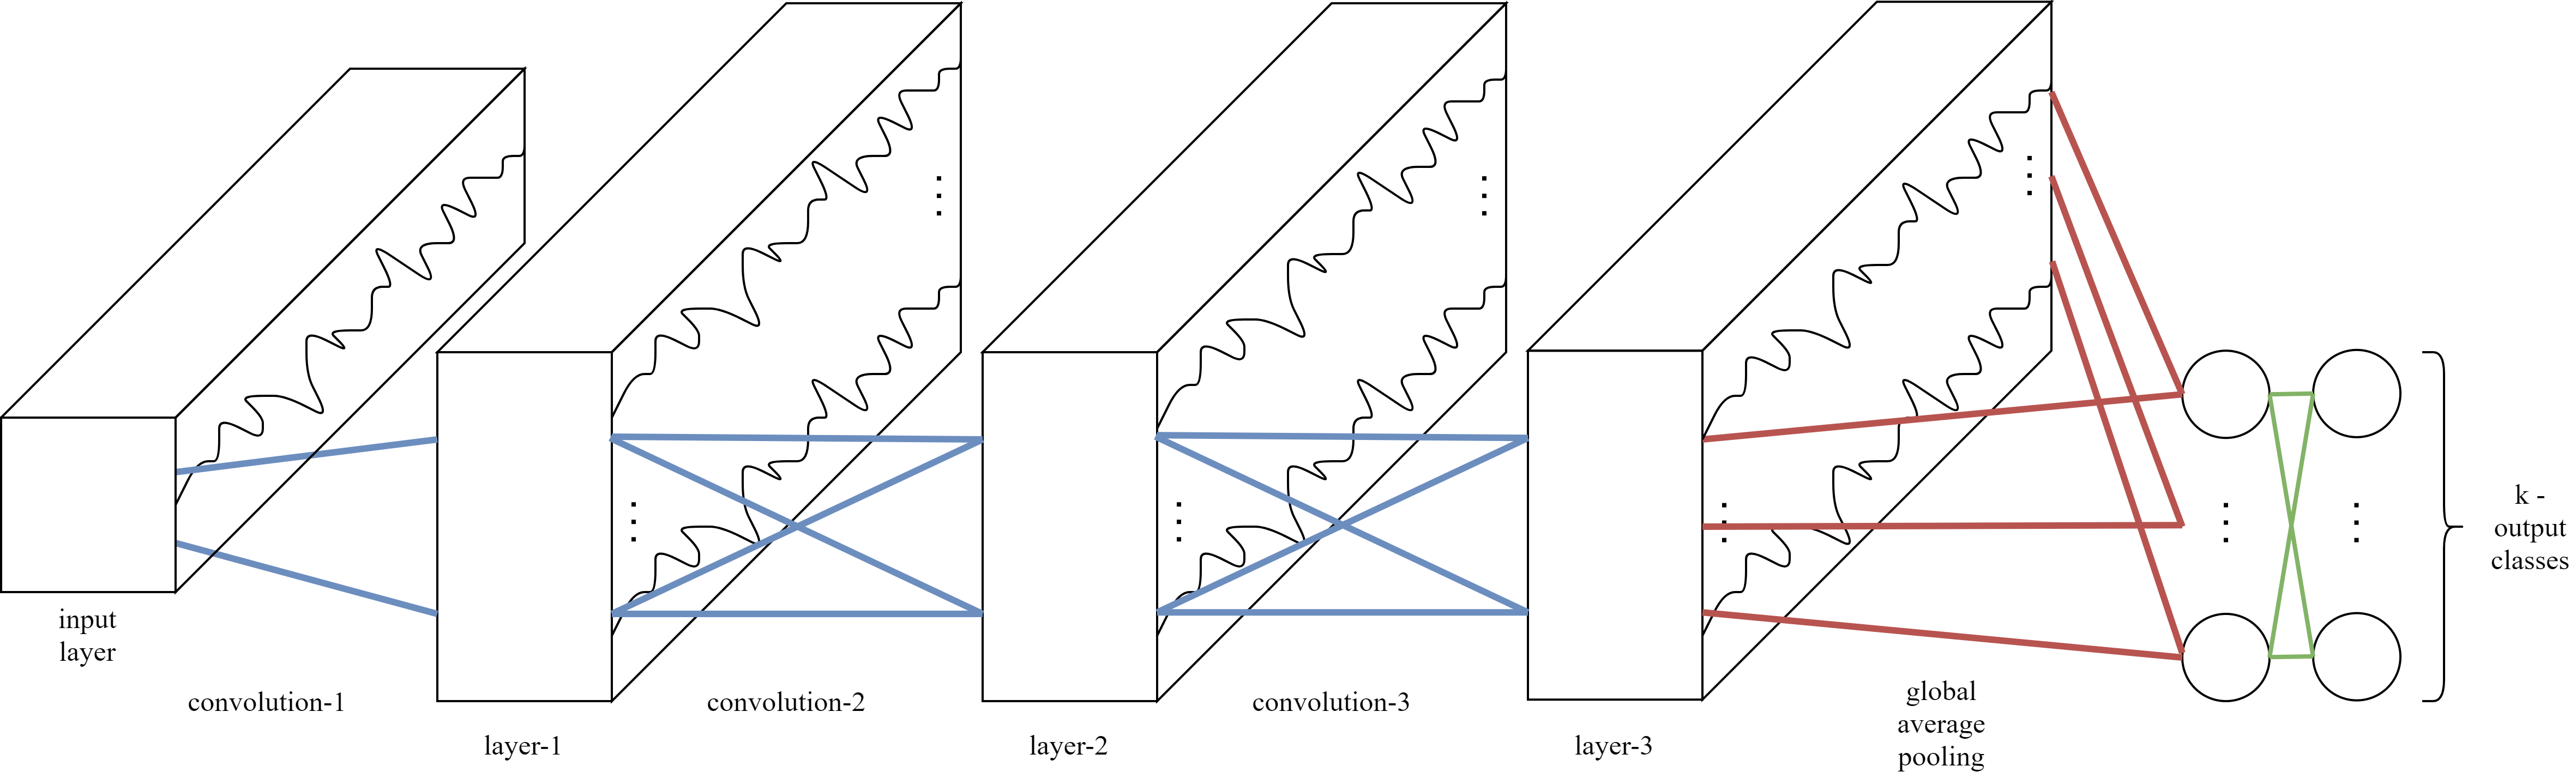
\includegraphics[width=\textwidth]{assets/CNN_basic_3_layers.png}
    
    \caption{Fully Convolutional Neural Network Architecture for Time Series Classification}
    \label{fig:cnn-layers}
\end{figure*}

\subsection{Echo-State Networks}
A further extension of deep learning models is the Recurrent Neural Network (RNN). This method is rarely used with time series data, with the exception of time series forecasting, due to three key factors.
\begin{itemize}
    \item the architecture is designed to predict an output for each element, so for time series, each time stamp \cite{langkvist2014}
    \item the models have a vanishing gradient problem when training on long time series \cite{pascanu2012}
    \item the models are hard to train and parallelise \cite{pascanu2012}
\end{itemize}
These problems led to the repurpose of Echo State Networks (ESNs) \cite{gallicchio2017}, which were first created for time series prediction in wireless communication channels \cite{jaeger2004}. They alleviate the vanishing gradient problem by eliminating the need to compute the gradient for hidden layers, also reducing the training time. These hidden layers are initialised randomly, and is known as the \textit{reservoir}, the core principal of an ESN, which is sparsely connected to an RNN. Consider an ESN with input dimensionality $M$, neurons in the reservoir $N_r$, and output dimensionality $K$. Letting $X(t), I(t), \hat{Y}(T)$ denote the multivariate time series, hidden state and output activity for time $t$ respectively. Formally the hidden state is:
\begin{equation}\label{eq:esn}
    I(t) = f(W_{\text{in}}X(t) + W I(t-1)) \ \big\rvert \ \forall \ t \in [1, T]
\end{equation}
where $f$, again, is the activation function, but usually ESNs use elementwise $\tanh$. With the output calculated by
\begin{equation}\label{eq:esn-output}
    \hat{Y}(t) = W_{\text{out}}I(t)
\end{equation}
thus classifying each time series element. Figure \ref{fig:esn-layers} demonstrates an example ESN for univariate time series classification, to be classified into $k$ classes.

\begin{figure}[h]
    \centering
    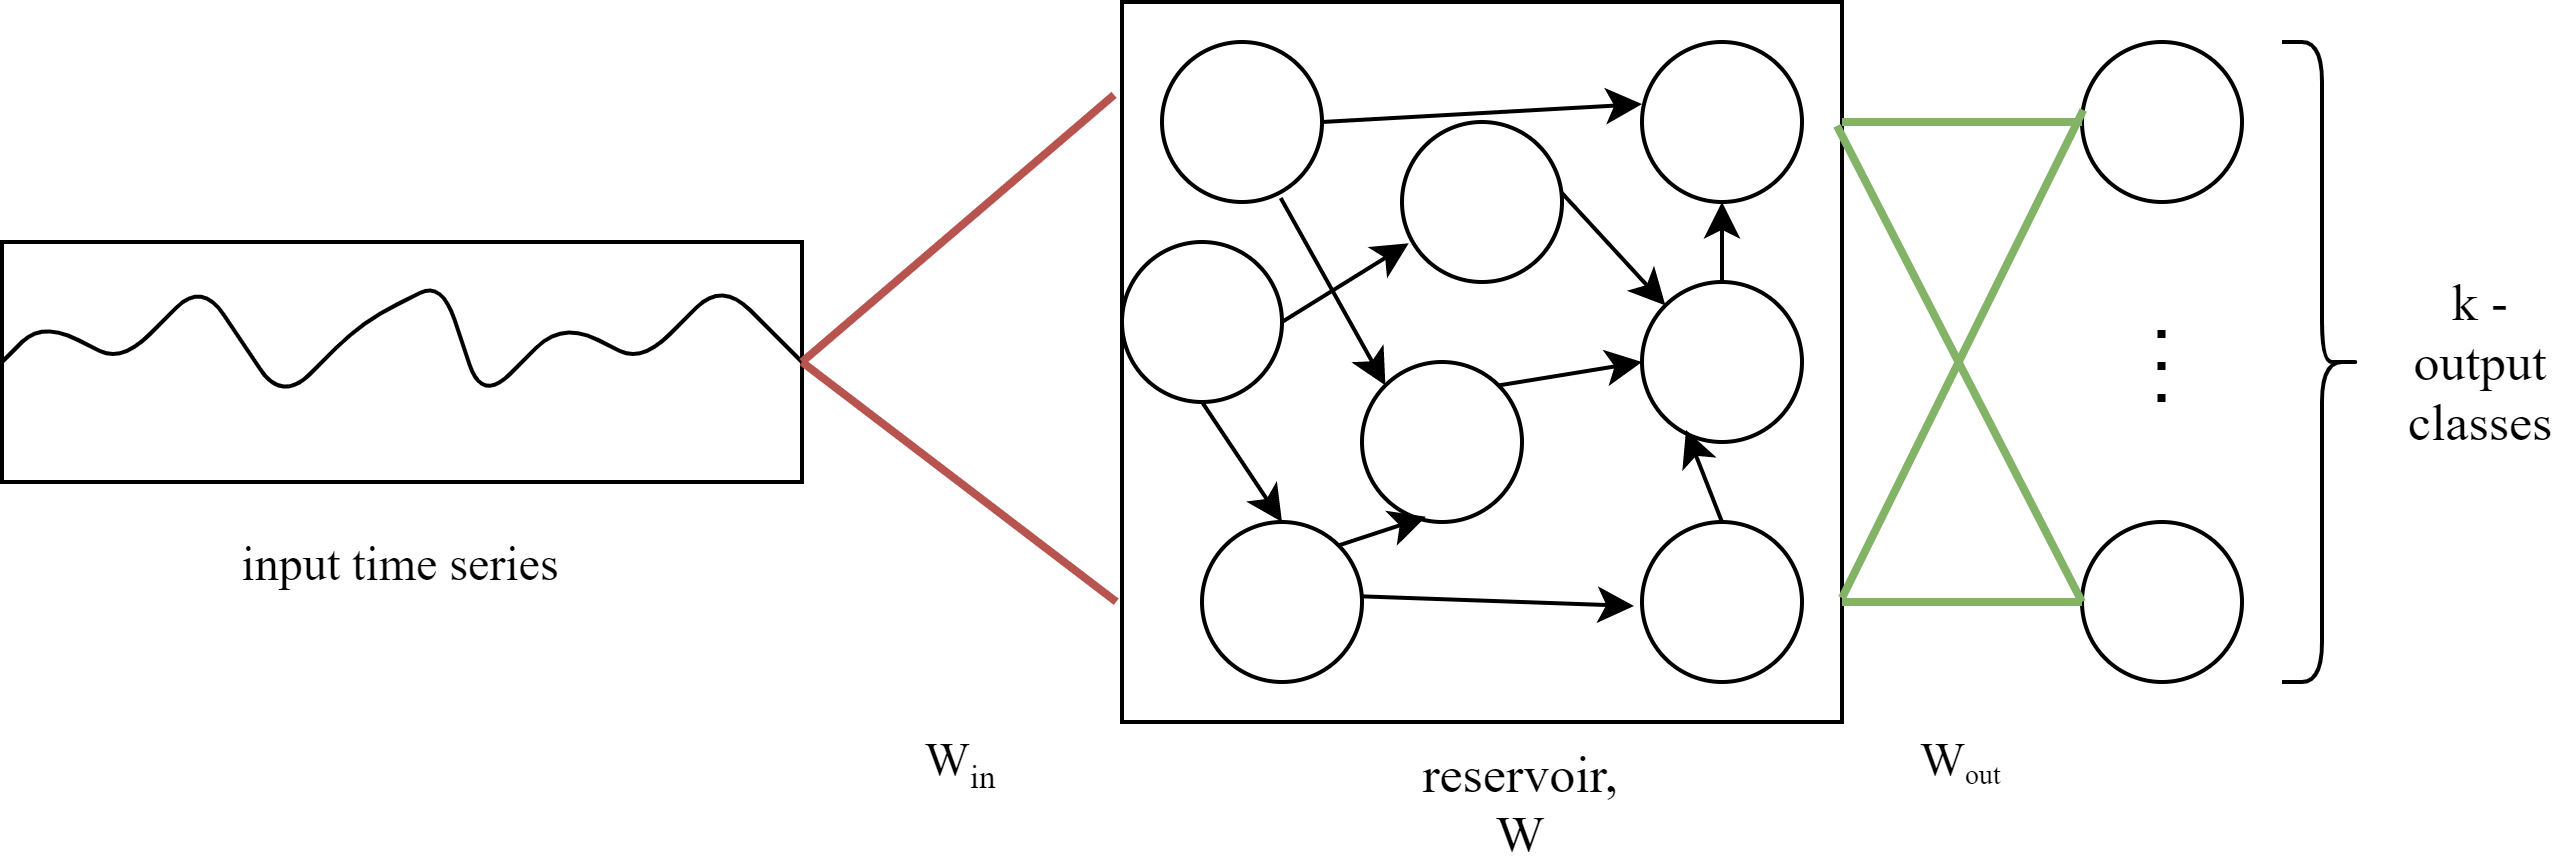
\includegraphics[width=3.5in]{assets/ESN_example.png}
    
    \caption{Echo State Network Architecture for Time Series Classification}
    \label{fig:esn-layers}
\end{figure}


\subsection{Approaches}
The approaches this analysis will consider are presented in Table \ref{tab:methods-architecture-1}, and they are further described in Table \ref{tab:methods-architecture-2}.

\begin{table*}[]
    \renewcommand{\arraystretch}{1.3}
    \centering
    \caption{Method Architecture's hyperparameters for each method}
    \label{tab:methods-architecture-1}
    
    \begin{tabular}{lllllllll}
    \hline
    \multirow{2}{*}{Methods} & \multicolumn{8}{l}{Architecture}                                              \\ \cline{2-9} 
                             & Layers & Conv & Invar & Normalise & Pooling & Feature & Activate & Regularise \\ \hline
    MLP                      & 4      & 0    & 0     & None      & None    & FC      & ReLU     & Dropout    \\
    ResNet                   & 11     & 9    & 10    & Batch     & None    & GAP     & ReLU     & None       \\
    Encoder                  & 5      & 3    & 4     & Instance  & Max     & Att     & PReLU    & Dropout    \\
    MCNN                     & 4      & 2    & 2     & None      & Max     & FC      & ReLU     & None       \\
    t-LeNet                  & 4      & 2    & 2     & None      & Max     & FC      & ReLU     & None       \\ \hline
    \end{tabular}
    
\end{table*}

\begin{table*}[]
    \renewcommand{\arraystretch}{1.3}
    \centering
    \caption{Optimisation hyperparameters for each method}
    \label{tab:methods-architecture-2}
    
    \begin{tabular}{llllllll}
    \hline
    \multirow{2}{*}{Methods} & Architecture &          &         &        &       &               &       \\ \cline{2-8} 
                             & Algorithm    & Valid    & Loss    & Epochs & Batch & Learning Rate & Decay \\ \hline
    MLP                      & AdaDelta     & Train    & Entropy & 500    & 16    & 1.0           & 0.0   \\
    ResNet                   & Adam         & Train    & Entropy & 500    & 16    & 0.001         & 0.0   \\
    Encoder                  & Adam         & Train    & Entropy & 100    & 12    & 0.00001       & 0.0   \\
    MCNN                     & Adam         & Split 20 & Entropy & 500    & 256   & 0.1           & 0.0   \\
    t-LeNet                  & Adam         & Train    & Entropy & 500    & 256   & 0.01          & 0.005 \\ \hline
    \end{tabular}
    
\end{table*}

\section{Experimental Setup}

\subsection{Datasets}
This paper considers 4 datasets, shown in Table \ref{tab:datasets}, 3 of these are from the UCR archive \cite{dau2019ucr} which contains 85 univariate time series datasets. The 4th dataset, which is also the key dataset of this report, is a subset of ECG5000

\begin{table}[]
    \renewcommand{\arraystretch}{1.3}
    \centering
    \caption{Dataset Properties}
    \label{tab:datasets}
    
    \begin{tabular}{lllll}
    \hline
    \multirow{2}{*}{Dataset} & \multicolumn{4}{l}{Properties}            \\ \cline{2-5} 
                             & Train Size & Test Size & Length & Classes \\ \hline
    ECG1                     & 4500       & 500       & 140    & 2       \\
    ECG200                   & 100        & 100       & 96     & 2       \\
    ECG5000                  & 500        & 4500      & 140    & 5       \\
    ECGfivedays              & 23         & 861       & 136    & 2       \\ \hline
    \end{tabular}

\end{table}

\subsubsection{ECG1}
This dataset is provided by TensorFlow and their method of construction is unclear. As described previously, this is the key dataset and a subset of ECG5000 where the classes have been modified from 5 classes provided by automated annotation to 2 classes, corresponding to abnormal rhythm or normal rhythm. This is provided as a single entity which must be split into test and train

\subsubsection{ECG200}
The dataset is from a PhD submission attempting to generalise feature extraction for strucurtal pattern recognition, \cite{olszewski2001}, Each series traces the electrical activity recorded during one heartbeat, and the 2 classes represent a normal heartbeat and a myocardial infarction. The properties are again described in Table \ref{tab:datasets}

\subsubsection{ECG5000}
The original dataset for this is a 20-hour long ECG from PhysioNet, where it is from BIDMC Congestive Heart Failure Database (chfdb) and it is record "chf07". It was originally published in \cite{Goldberger2000}. The data was pre-processed by \cite{Chen2014} in two steps (1) extract each heartbeat, (2) make each heartbeat equal length using interpolation. After this, 5000 heartbeats were randomly selected, the patient is known to have severe congestive heart failure and class values were obtained by automated annotation.

\subsubsection{ECGfivedays}
This dataset is from \cite{Chen2014}, in addition to ECG5000 and subsequently ECG1, it is data from a 67 year old male where the two classes are the date of recording, namely, 12/11/1990 or 17/11/1990 - it is nondescript what these dates represent.

\subsection{Pre-Processing}
All datasets have their labels extracted and the data is coerced into numeric form, with the labels, using sklearn one-hot encoding, converted to one hot vectors and an additional variable which stores the argmax of these vectors. Univariate datasets are then changed into multivariate problems with one dimension - this is then passed to the respective classifier.


\subsection{Experiments}
For each dataset, the 5 deep learning models (as in the previous section) are trained with 3 runs each. Each run uses the same test and train subsets, as this is done either externally in the case of datasets from UCR, or internally via a seeded test-train split, in the case of ECG1. Each run will generate different initial random weights, and so the 3 runs are averaged to reduce bias. In total there are 20 models, with 60 experiments (not including MCNN hyper-parameter searching). This was run on an Nvidia GTX 970, with 4GB of GDDR5. The total sequential running time was approximately 27 hours. Each method was implemented using the open source deep learning library Keras \cite{chollet2015keras}, with TensorFlow \cite{tensorflow2015} backend. Using the mean accuracy over the 3 runs \cite{grabocka2014}, the Friedman test is used to reject the null hypothesis then a pairwise post-hoc analysis - where the average rank comparison is replaced by a Wilcoxon signed-rank test with Holm's alpha correction. This is visualised using critical difference diagrams, where a thick horizontal line shows a group of classifiers that are not-significantly different in terms of accuracy.

\section{Results}

\begin{figure*}[h]
    \centering
    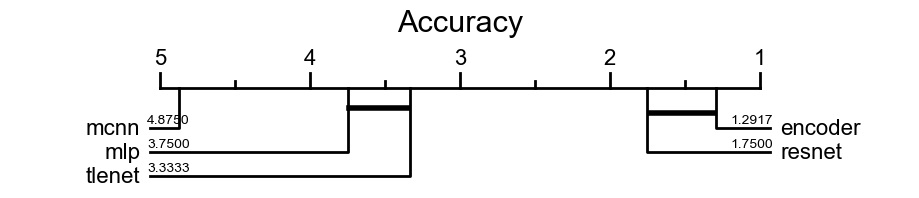
\includegraphics[width=\textwidth]{assets/all_models_all_runs.png}
    
    \caption{Critical Difference diagram showing pairwise statistical difference comparison of five deep learning classifiers on all datasets}
    \label{fig:wilcoxon-all-datasets}
\end{figure*}

\begin{figure}[h]
    \centering
    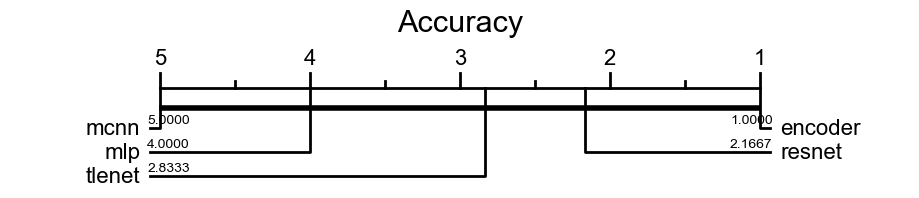
\includegraphics[width=3.5in]{assets/all_models_ecg1.png}
    
    \caption{Critical Difference diagram showing pairwise statistical difference comparison of five deep learning classifiers on the dataset \textit{ecg1}}
    \label{fig:wilcoxon-ecg1}
\end{figure}



\begin{figure}[h]
    \centering
    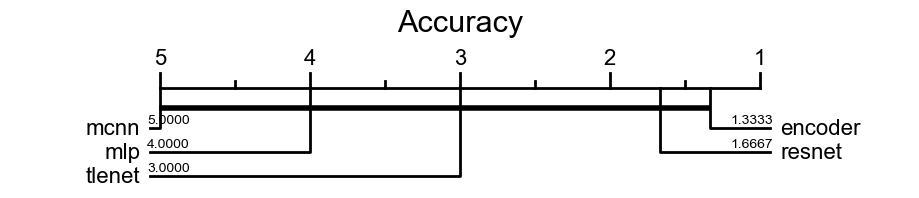
\includegraphics[width=3.5in]{assets/all_models_ecg5000.png}
    
    \caption{Critical Difference diagram showing pairwise statistical difference comparison of five deep learning classifiers on \textit{ecg5000}}
    \label{fig:wilcoxon-ecg5000}
\end{figure}



\begin{figure}[h]
    \centering
    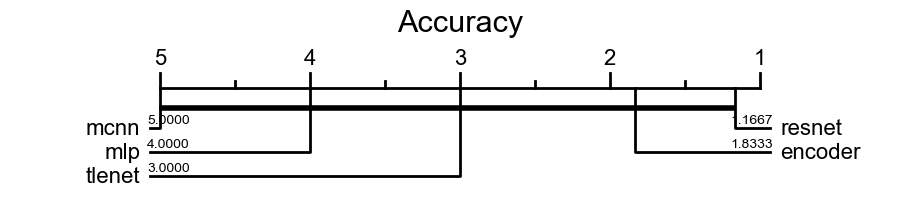
\includegraphics[width=3.5in]{assets/all_models_ecgfivedays.png}
    
    \caption{Critical Difference diagram showing pairwise statistical difference comparison of five deep learning classifiers on \textit{ecgfivedays}}
    \label{fig:wilcoxon-ecgfivedays}
\end{figure}

\begin{figure}[h]
    \centering
    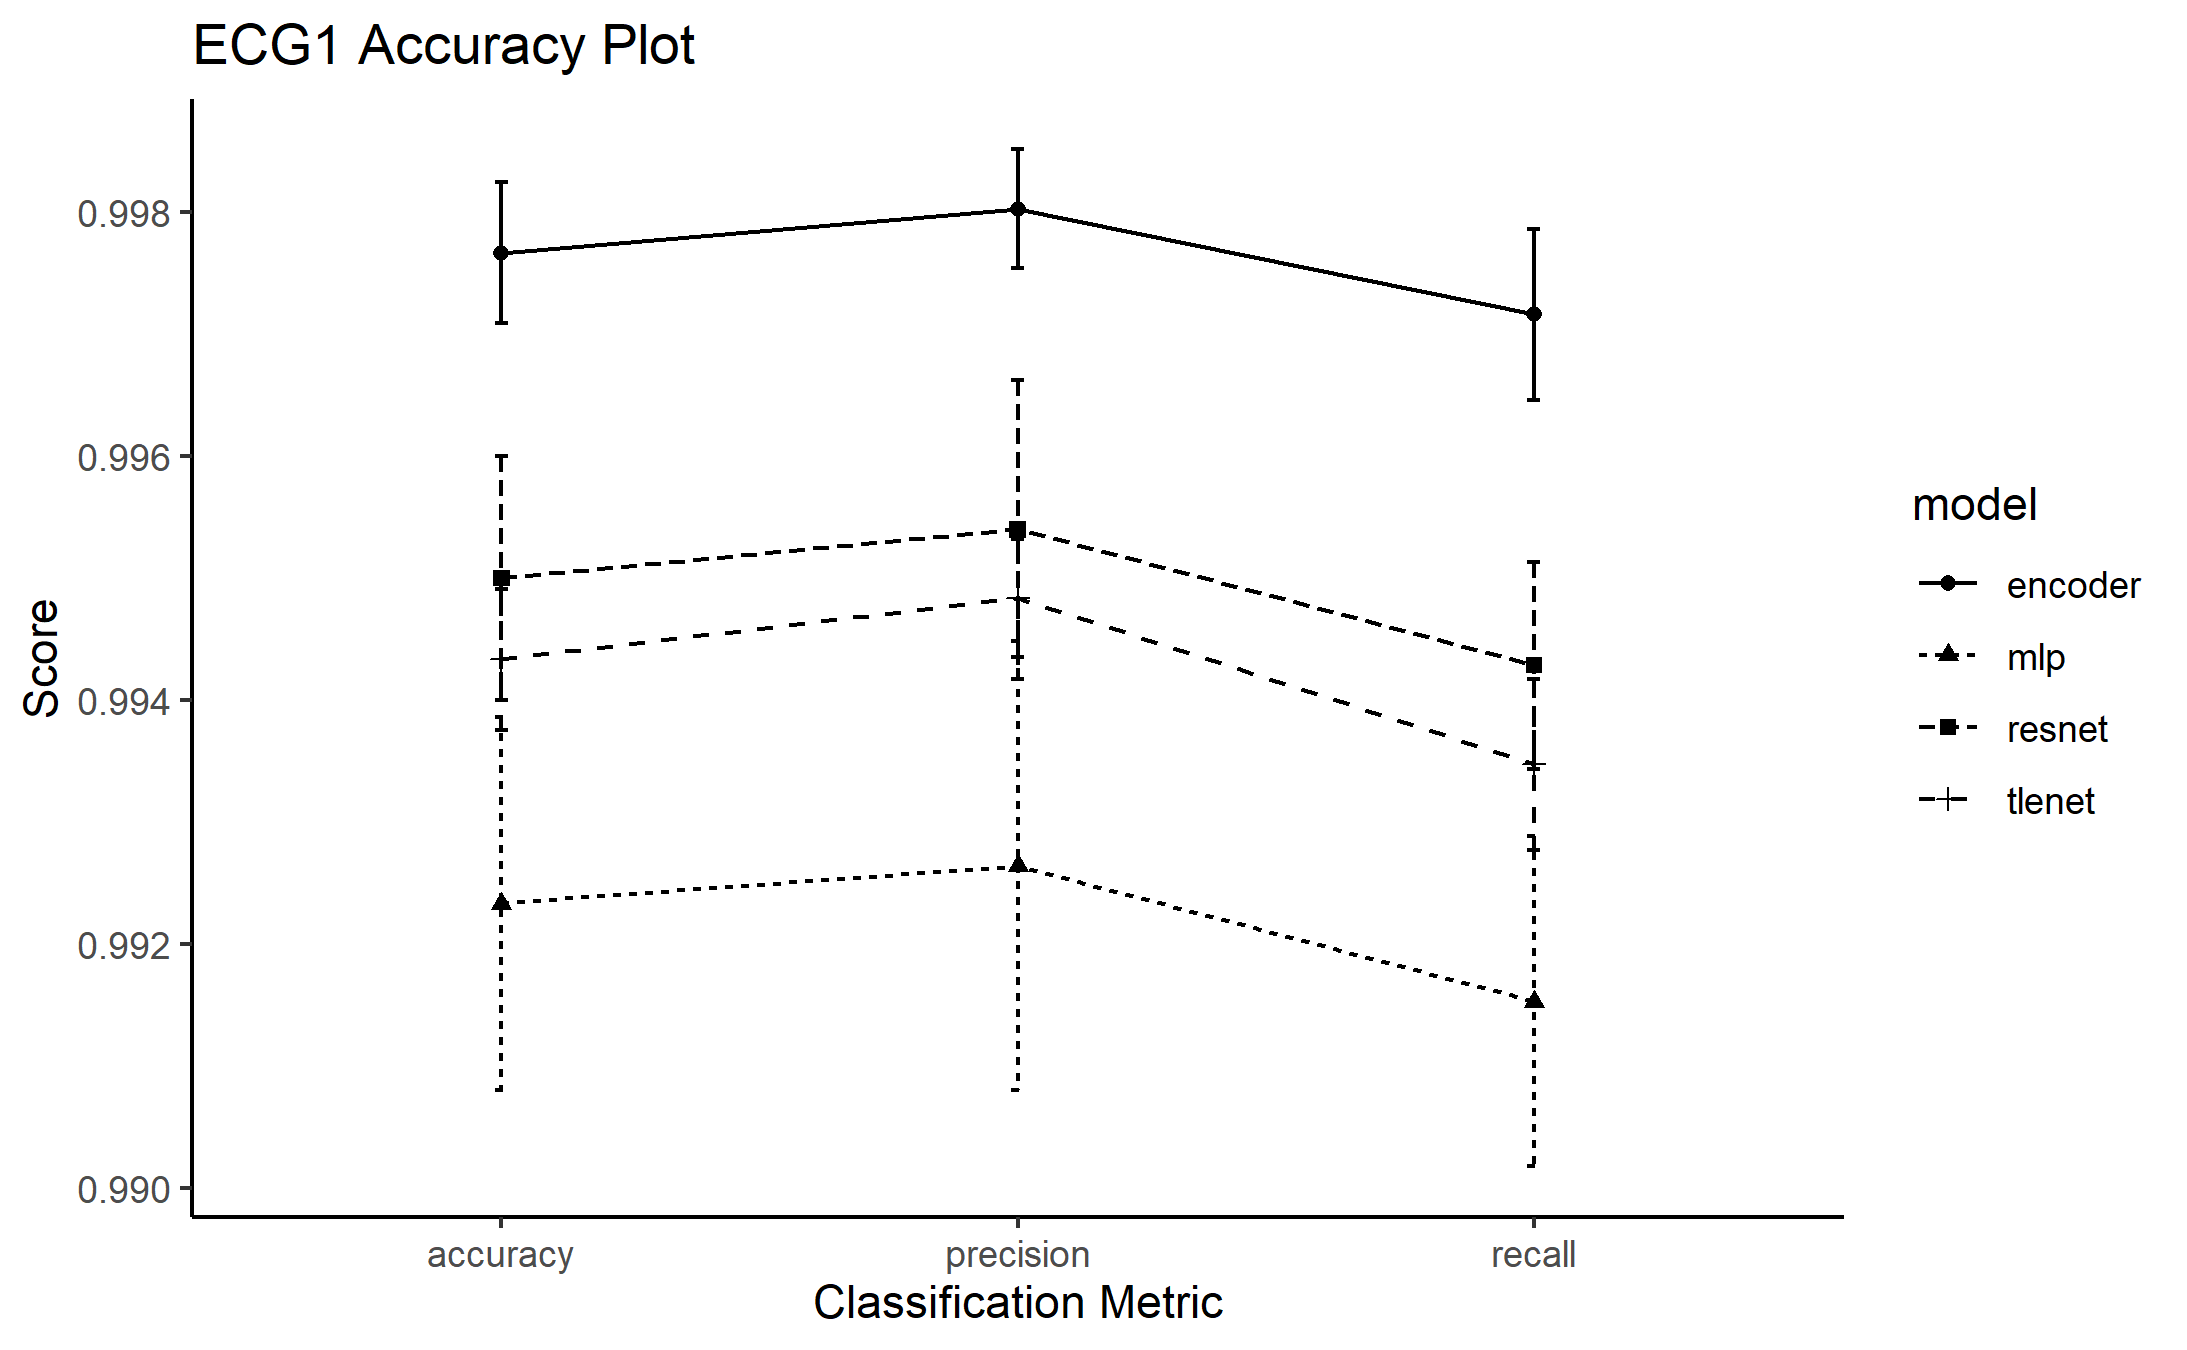
\includegraphics[width=3.5in]{assets/ecg1_accuracy_plot.png}
    
    \caption{Classification Metics (with average, sd error bars) for each model for \textit{ECG1}}
    \label{fig:ecg1-accuracy}
    
\end{figure}

\begin{figure}[h]
    \centering
    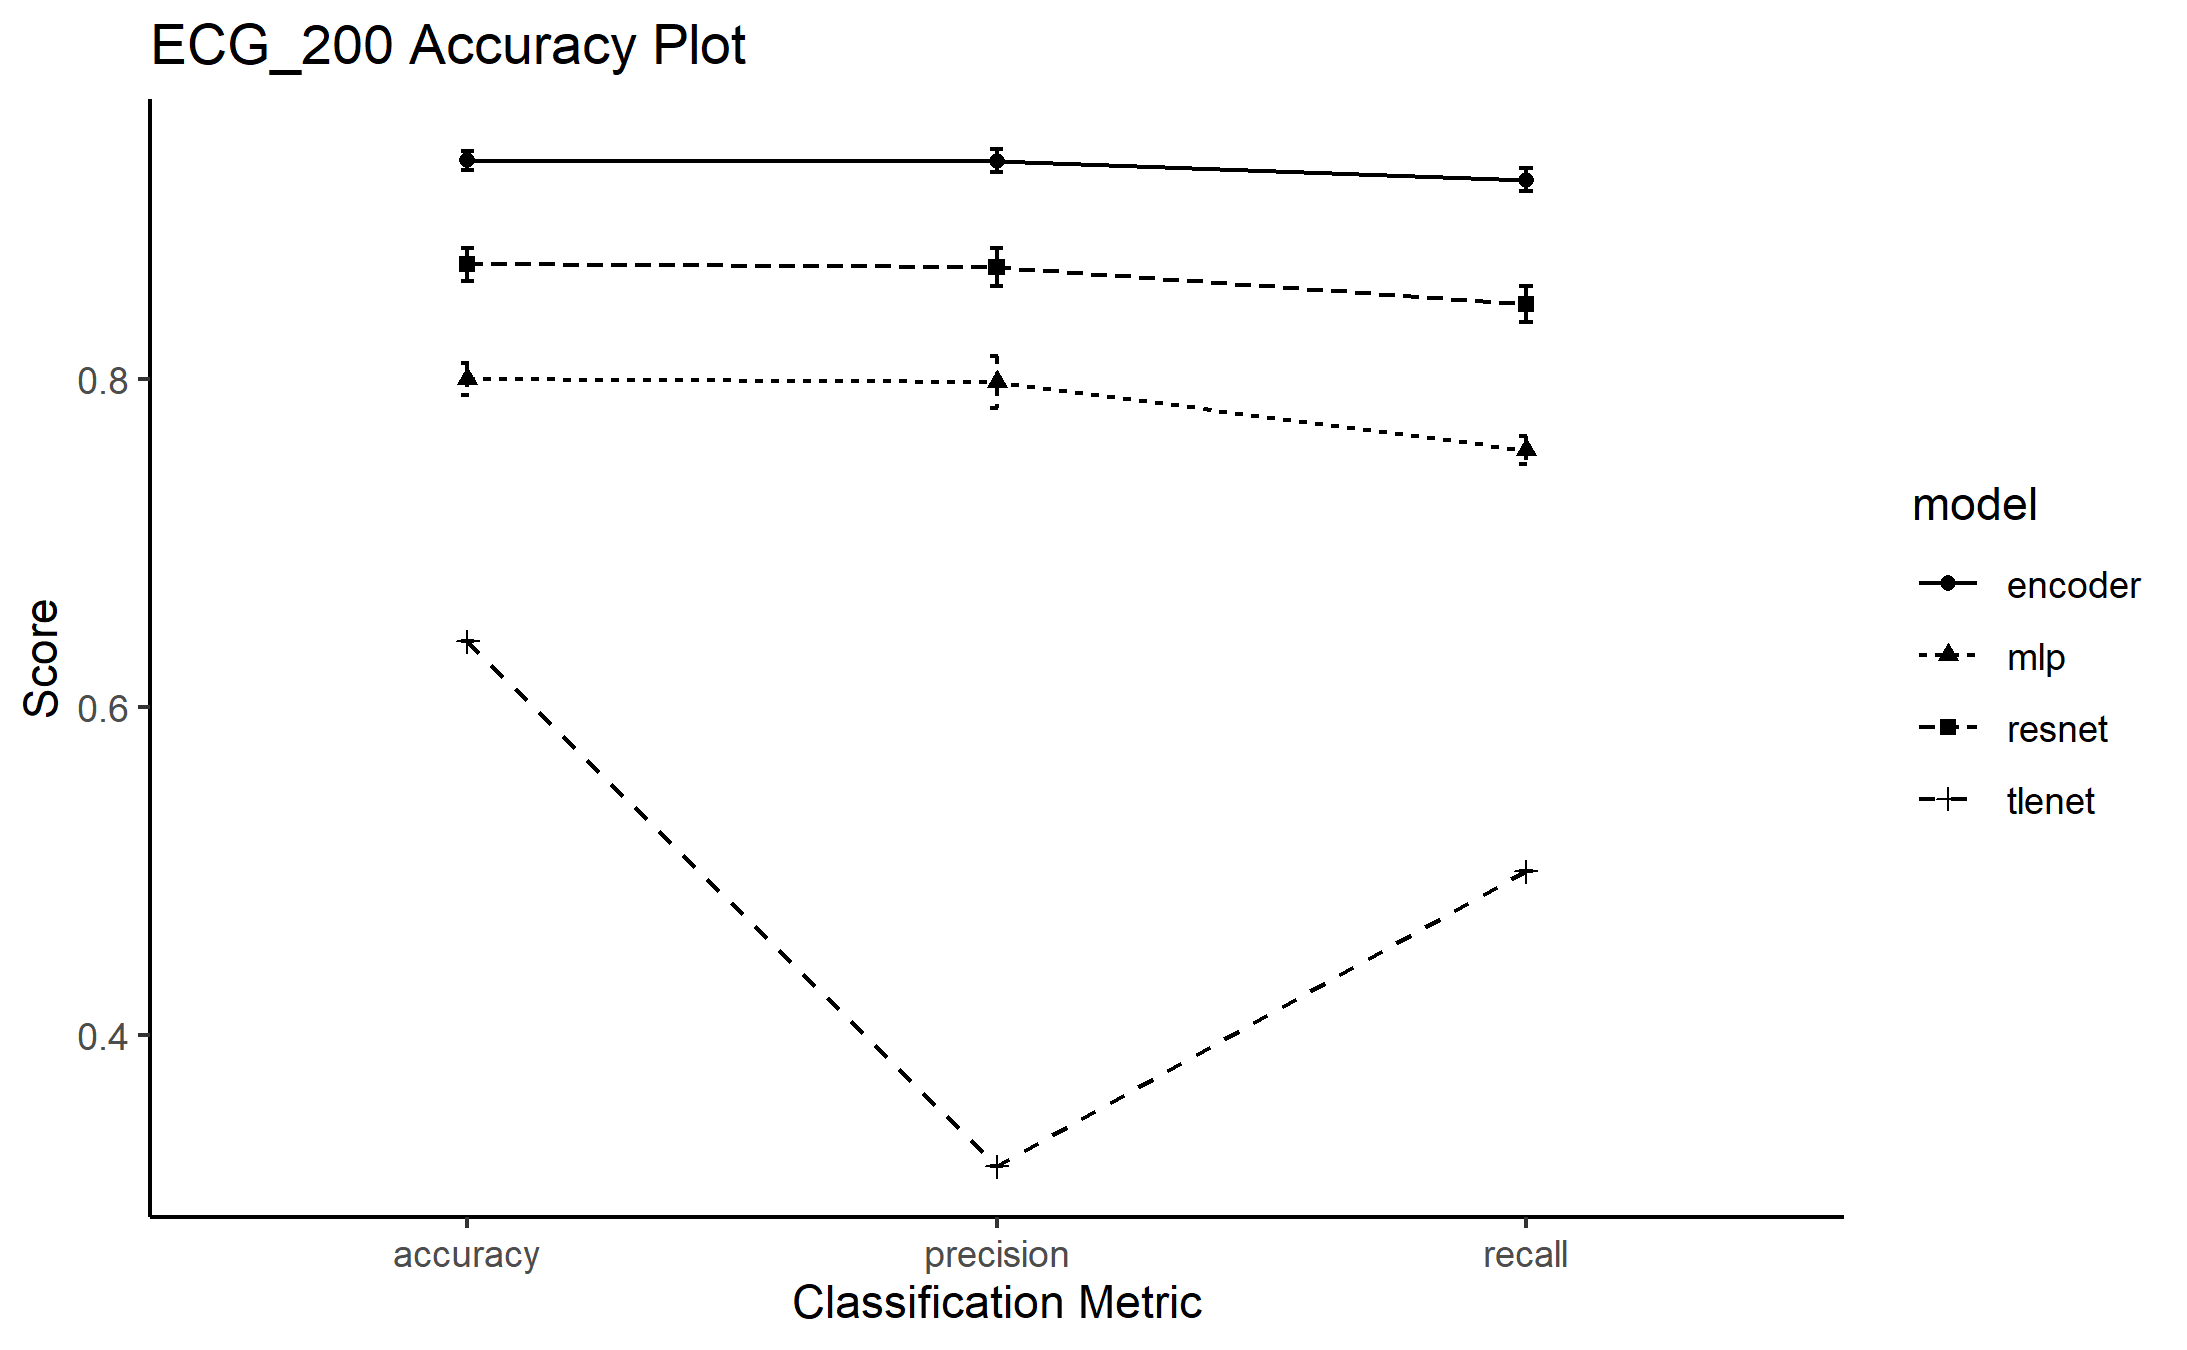
\includegraphics[width=3.5in]{assets/ecg200_accuracy_plot.png}
    
    \caption{Classification Metics (with average, sd error bars) for each model for \textit{ECG200}}
    \label{fig:ecg200-accuracy}
    
\end{figure}

\begin{figure}[h]
    \centering
    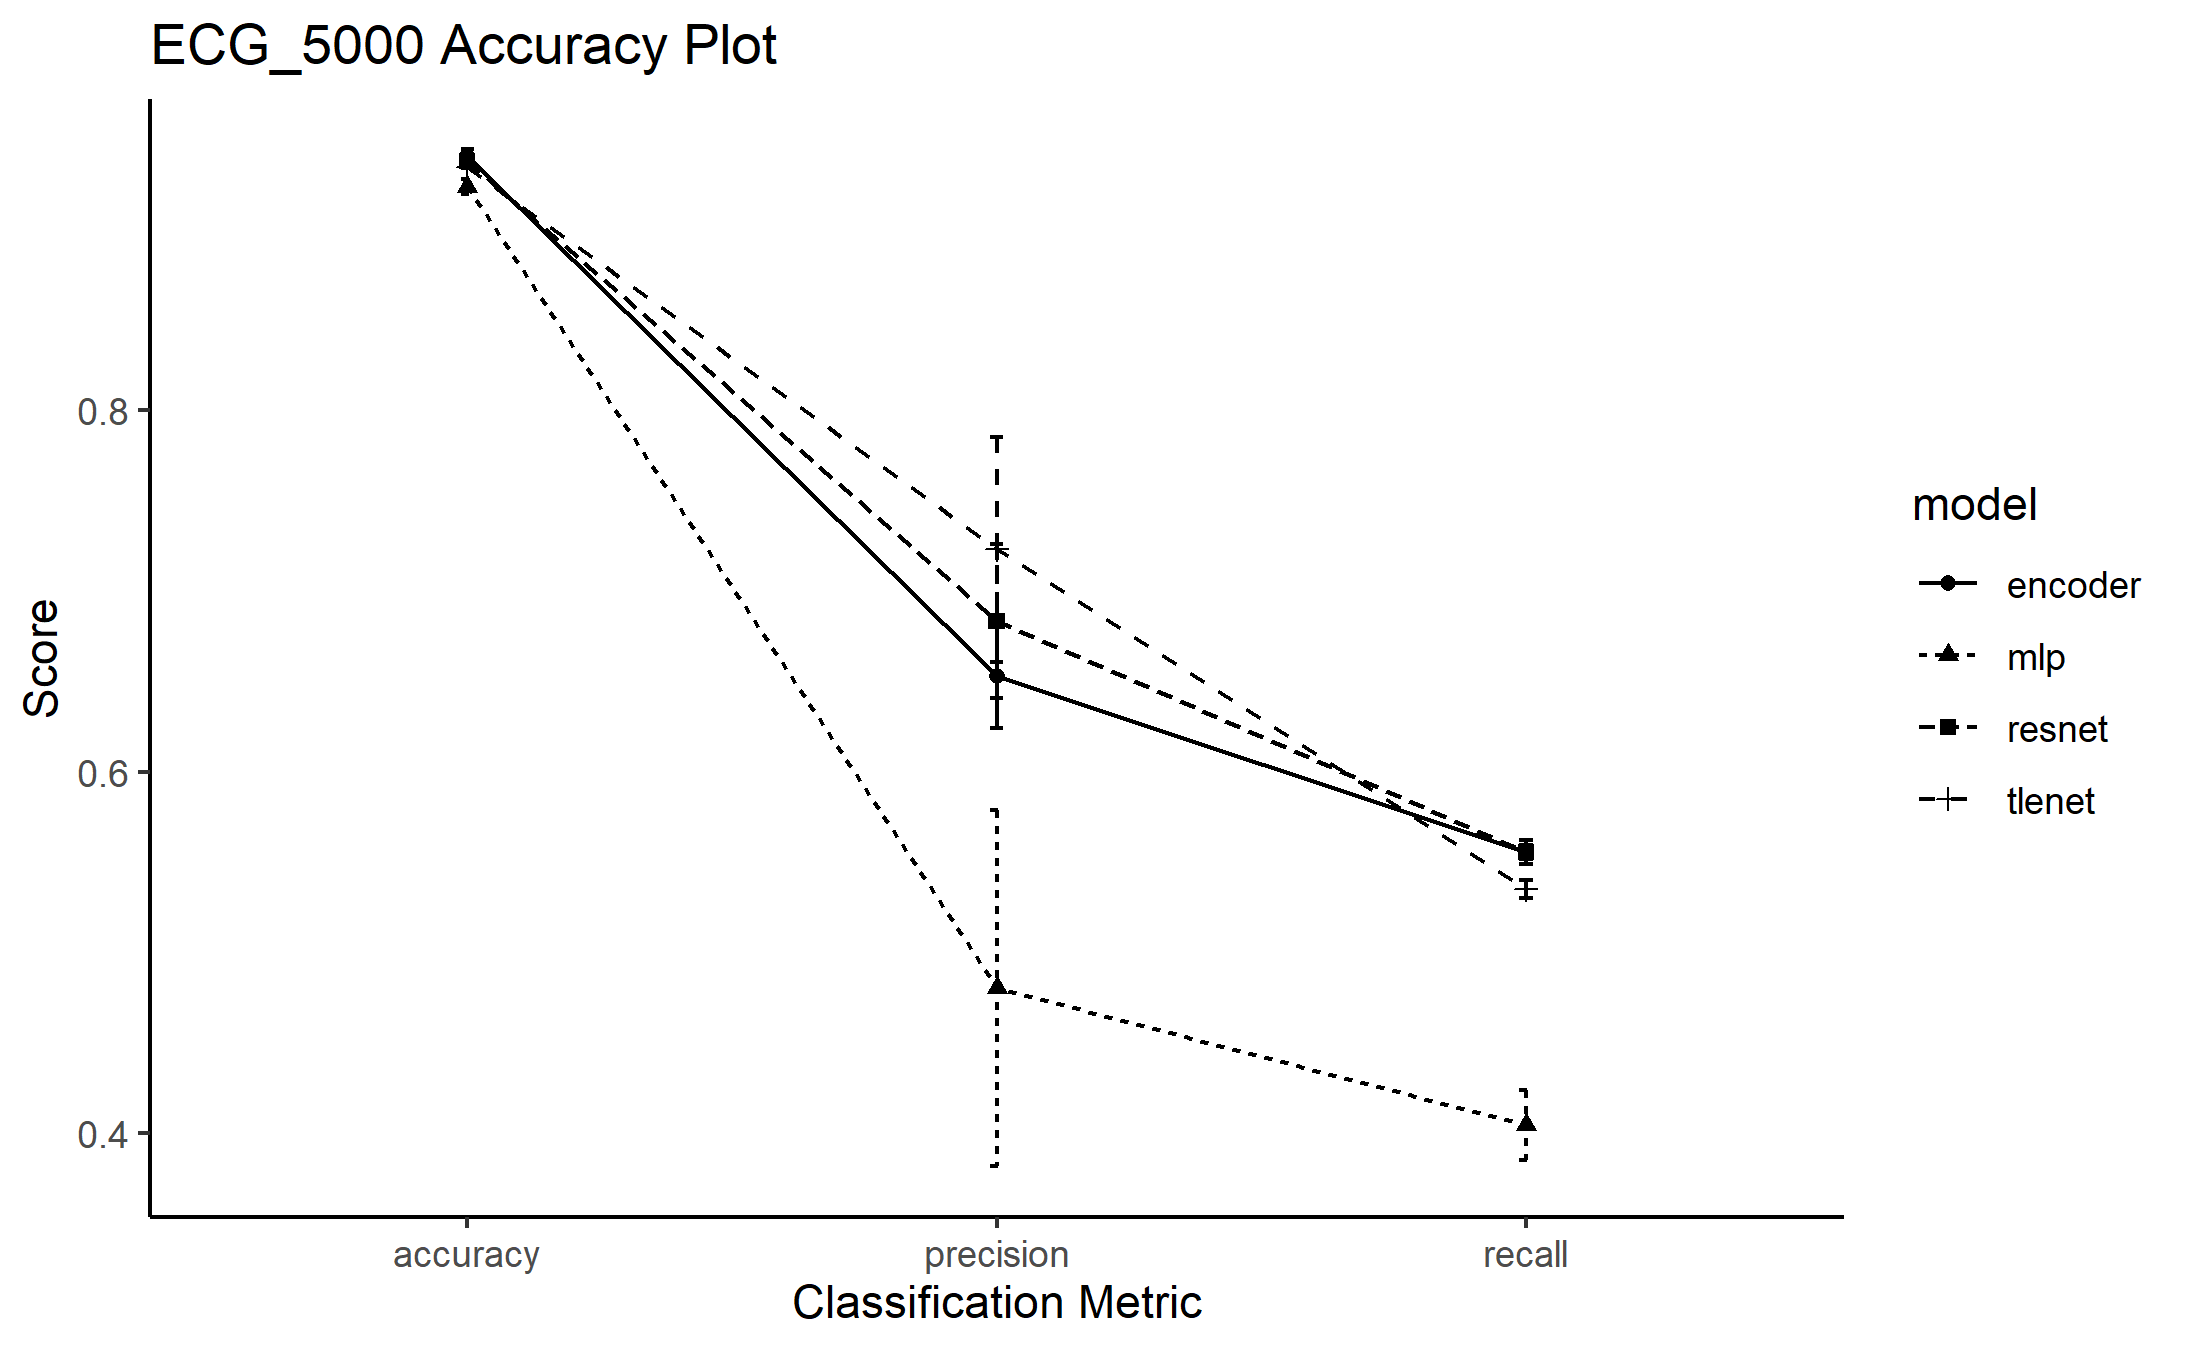
\includegraphics[width=3.5in]{assets/ecg5000_accuracy_plot.png}
    
    \caption{Classification Metics (with average, sd error bars) for each model for \textit{ECG5000}}
    \label{fig:ecg5000-accuracy}
    
\end{figure}

\begin{figure}[h]
    \centering
    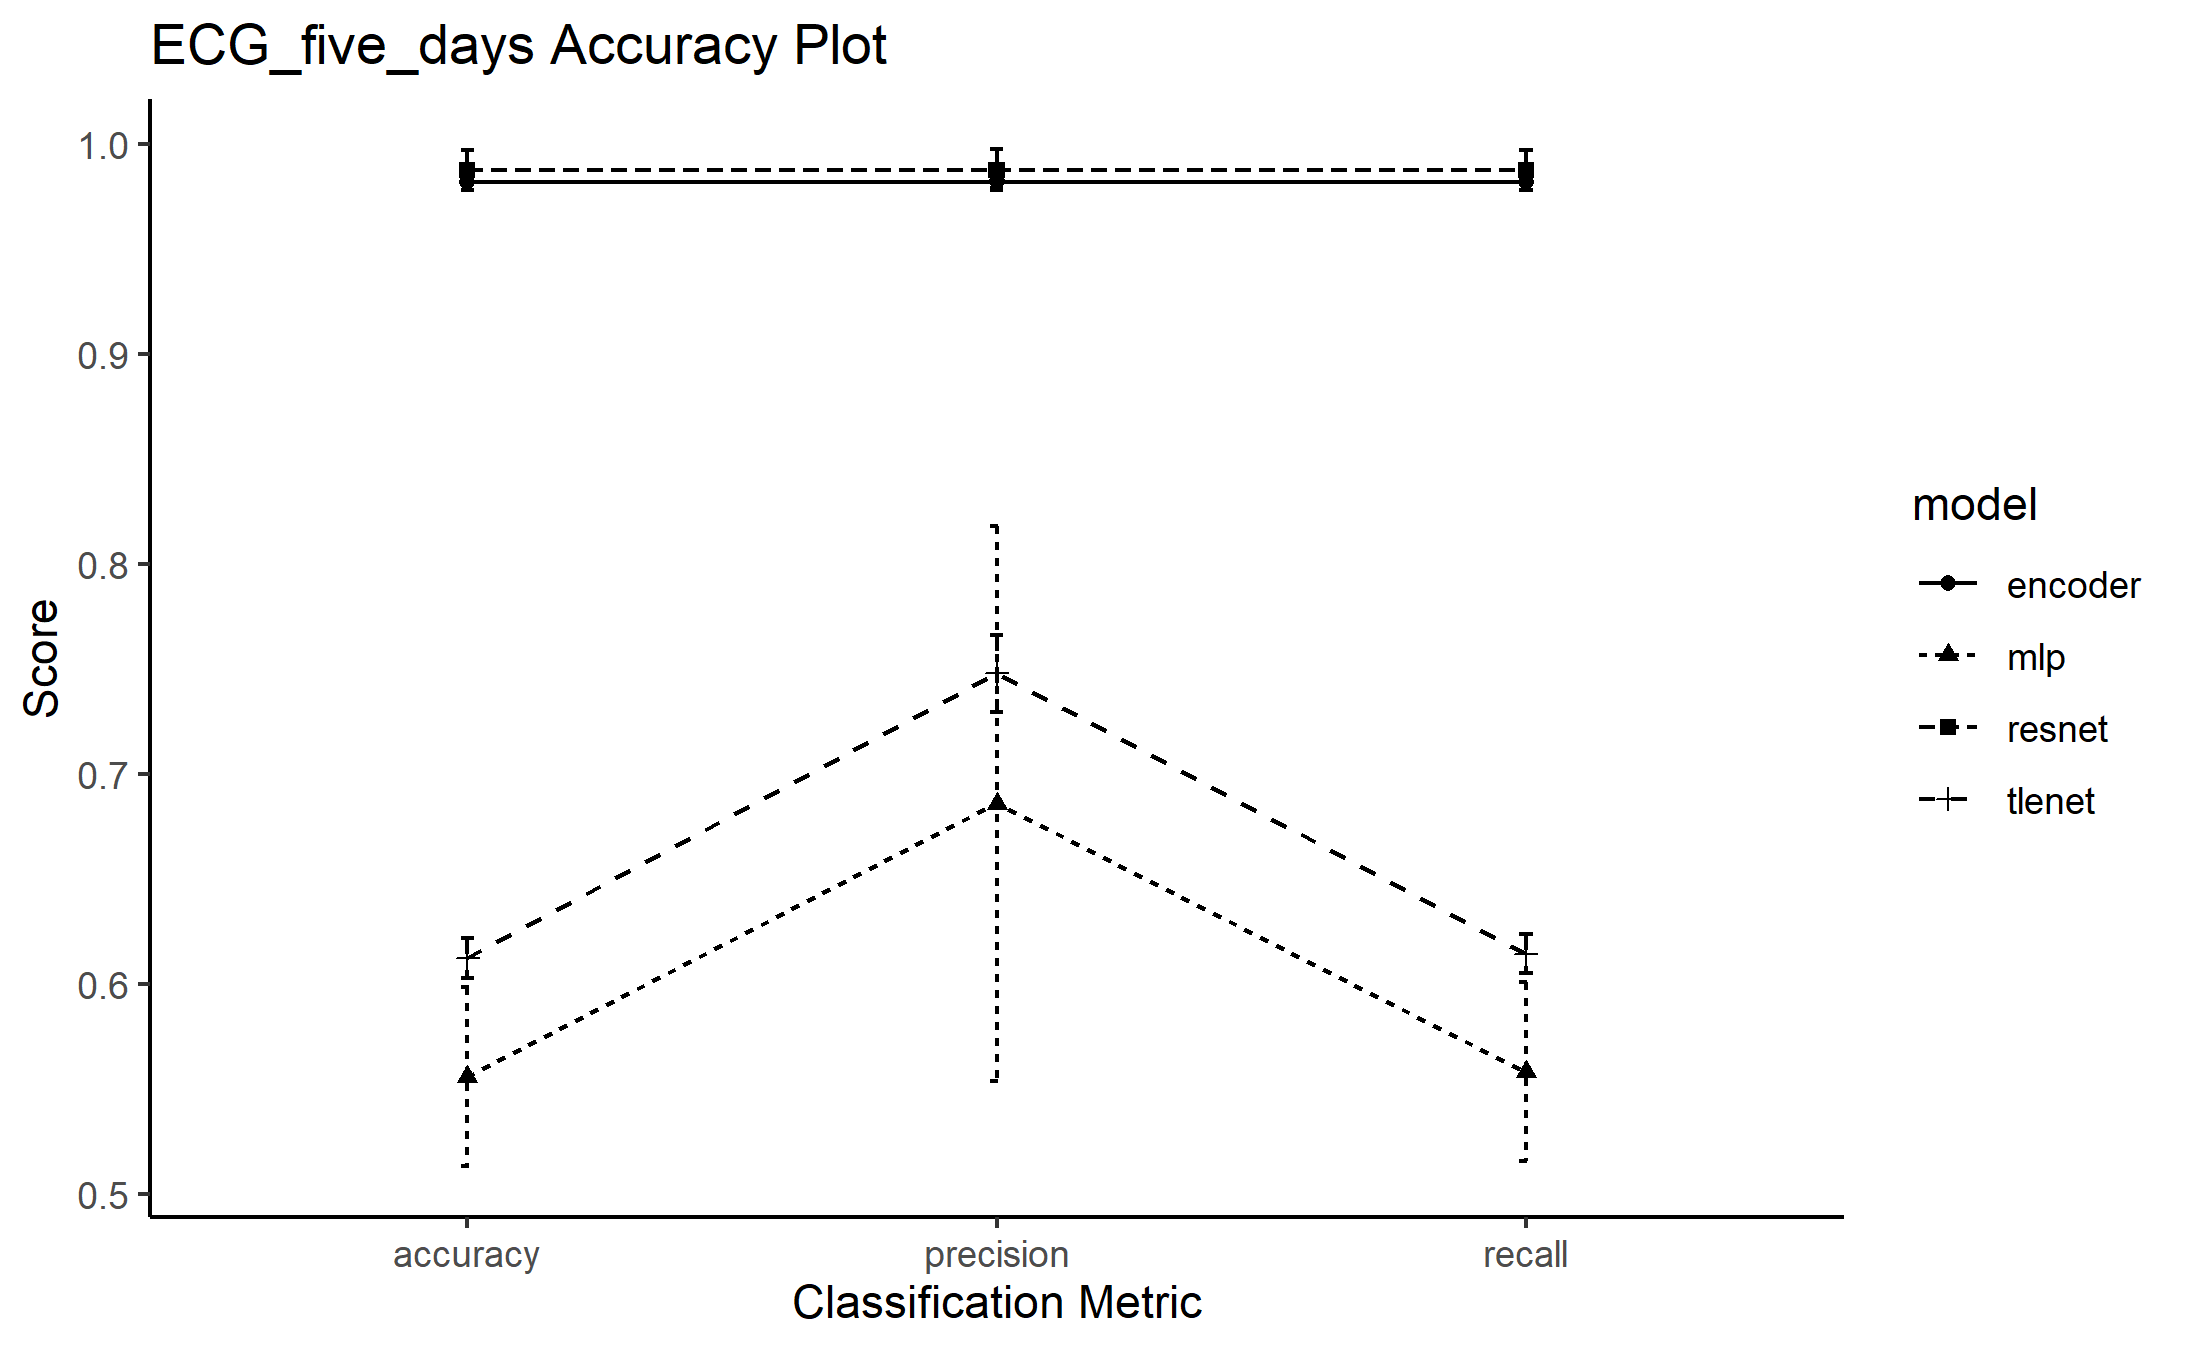
\includegraphics[width=3.5in]{assets/ecgfivedays_accuracy_plot.png}
    
    \caption{Classification Metics (with average, sd error bars) for each model for \textit{ECGfivedays}}
    \label{fig:ecgfivedays-accuracy}
    
\end{figure}

\begin{figure}[h]
    \centering
    \subfloat[MLP]{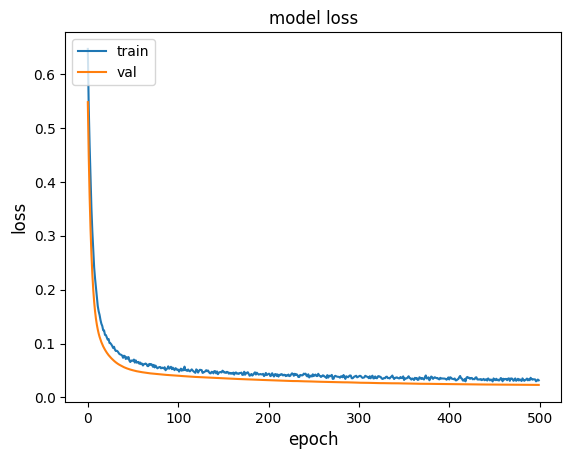
\includegraphics[width=2.5in]{assets/ecg1_loss/mlp.png}%
    \label{fig:loss-mlp}}
    \hfil
    \subfloat[Encoder]{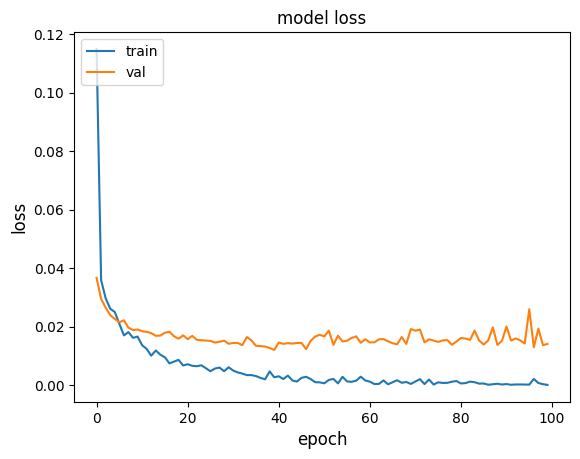
\includegraphics[width=2.5in]{assets/ecg1_loss/encoder.png}%
    \label{fig:loss-encoder}}
    \caption{Loss Metrics for (a) MLP and (b) Encoder for dataset \textit{ECG1} across epochs}
    \label{fig:loss-1}
\end{figure}

\begin{figure}[h]
    \centering
    \subfloat[t-LeNet]{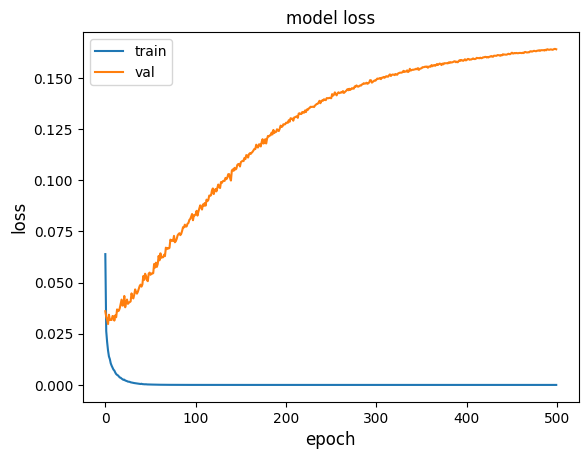
\includegraphics[width=2.5in]{assets/ecg1_loss/tlenet.png}%
    \label{fig:loss-tlenet}}
    \hfil
    \subfloat[ResNet]{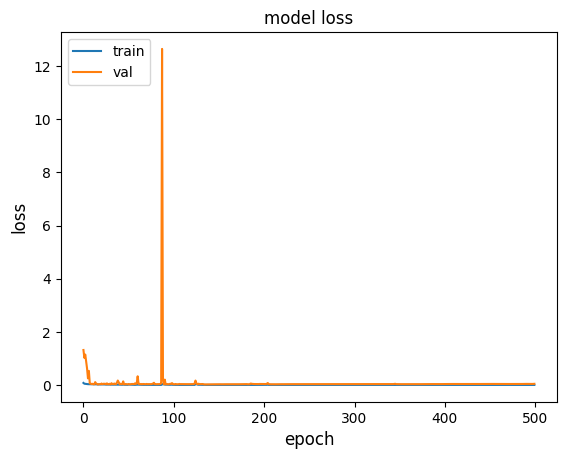
\includegraphics[width=2.5in]{assets/ecg1_loss/resnet.png}%
    \label{fig:loss-resnet}}
    \caption{Loss Metrics for (a) ResNet and (b) t-LeNet for dataset \textit{ECG1} across epochs}
    \label{fig:loss-2}
\end{figure}

All experiments from the previous section were compiled into a single table from which all analysis is performed and selected via R, except the critical difference diagram creation which is performed in python \cite{IsmailFawaz2018deep}. The critical difference diagram for all 4 datasets is shown in Figure \ref{fig:wilcoxon-all-datasets}. There are 3 bands of classifiers, the Encoder and ResNet outperform all other models with average ranks of 1.2917 and 1.7500 repectively. These classifers are consistently ranked 1st and 2nd for all datasets and significantly outperform the FCN architecture, which contrasts previous results where FCN has been found to outperform ResNet in most scenarios - this is reinforced in the validation of larger archives supporting this \cite{IsmailFawaz2018deep}. The middle band consists of MLP and t-LeNet, with average ranks of 3.7500 and 3.3333 respectively - MLP is not a widely used method as it has been improved to give increased accuracy at decreased computation, it is however, an important baseline method. The t-LeNet architecure outperformed expectations by being the middle method, previous experimentation has shown that the t-LeNet suffer from low accuracy problems with time series data due to their time slicing-majority voting scheme classification method. Additionally MCNN suffers from this problem, and was expected to perform somewhat poorly.



The primary dataset of this comparative analysis is \textit{ecg1}, the critical difference diagram is shown in Figure \ref{fig:wilcoxon-ecg1} - it returns similar results to the all-datasets version in Figure \ref{fig:wilcoxon-all-datasets} - with the notable exception that there is no statistical significance between the results. This is because all methods are able to quickly gain an accuracy $ \approx1.000$, but it must be added that all models see their peak performance in the last $\approx10$ epochs, their accuracies can be seen in Figure \ref{fig:ecg1-accuracy}, these also have low loss values, seen in Figures \ref{fig:loss-1}, \ref{fig:loss-2}, in addition to good precision and recall values, however notably Encoder scores the best, followed by ResNet and MLP - whom score very closely - with t-LeNet attaining the lowest scores and also largest error margins. All the error margins for \textit{ECG1} can be attributed
to having a smaller test set, as well as the random starting point. This is not the case for \textit{ECG200}, which has a far larger test case, with the error margins for accuracy, precision and recall shown in Figure \ref{fig:ecg200-accuracy}, t-LeNet again scores very poorly, with the other models performing admirably, and Encoder returning the strongest results. The critical difference diagram for \textit{ECG200} could not be created due to results being within a too small error margin. The critical difference diagram for \textit{ECG5000} is shown in Figure \ref{fig:wilcoxon-ecg5000} and returns the same as the previous two with Encoder and ResNet performing the strongest however, as shown in the thick black line, the difference is statistically insignificant, the classification metrics are in Figure \ref{fig:ecg5000-accuracy} where high accuracy are seen for all methods, however very low precision and recall values suggest this model is over-fitted, as well as large error margins for the precision metric. There is similar to \textit{ECGfivedays} which sees Encoder and ResNet attaining extremely strong scores of $ \approx 1$ for accuracy, precision and recall, as seen in Figure \ref{fig:ecgfivedays-accuracy}. t-LeNet and MLP are very weak, having low accuracy and low recall, however according to the critical difference diagram, in Figure \ref{fig:wilcoxon-ecgfivedays}, the difference is statistically insignificant.




\section{Conclusion}
This analysis presented recent successful architecures for Time Series Classification, it was described how Deep Neural Networks are categorised and selected methods were mathematically defined. Five end-to-end methods were implemented , training them with 4 ECG datasets - 1 primary and 3 secondary datasets. The results show that Encoder and ResNet produce great results and outperform previous attempts to use deep learning to classify ECG data, with Encoder scoring an average accuracy of 96\%, additionally, this accuracy is far above the average cardiologist \cite{rajpurkar2017}. Although this comparative analysis extensively analysed methods and ECG data, further study is required regarding data augmentation, and transferability of learning. Additionally an extensive study of computation time, and expensive functions is required to enable these methods to process more data efficiently. In conclusion, with ECG data becoming more easily shared within healthcare systems, leveraging deep learning architectures capable of learning from massess of data with ease, deep learning is prime position to enable healthcare providers to implement their own analysis to automatically recognise heart conditions that cardiologists do not have the time to evaluate.


% An example of a floating figure using the graphicx package.
% Note that \label must occur AFTER (or within) \caption.
% For figures, \caption should occur after the \includegraphics.
% Note that IEEEtran v1.7 and later has special internal code that
% is designed to preserve the operation of \label within \caption
% even when the captionsoff option is in effect. However, because
% of issues like this, it may be the safest practice to put all your
% \label just after \caption rather than within \caption{}.
%
% Reminder: the "draftcls" or "draftclsnofoot", not "draft", class
% option should be used if it is desired that the figures are to be
% displayed while in draft mode.
%
%\begin{figure}[!t]
%\centering
%\includegraphics[width=2.5in]{myfigure}
% where an .eps filename suffix will be assumed under latex, 
% and a .pdf suffix will be assumed for pdflatex; or what has been declared
% via \DeclareGraphicsExtensions.
%\caption{Simulation results for the network.}
%\label{fig_sim}
%\end{figure}

% Note that the IEEE typically puts floats only at the top, even when this
% results in a large percentage of a column being occupied by floats.


% An example of a double column floating figure using two subfigures.
% (The subfig.sty package must be loaded for this to work.)
% The subfigure \label commands are set within each subfloat command,
% and the \label for the overall figure must come after \caption.
% \hfil is used as a separator to get equal spacing.
% Watch out that the combined width of all the subfigures on a 
% line do not exceed the text width or a line break will occur.
%
%\begin{figure*}[!t]
%\centering
%\subfloat[Case I]{\includegraphics[width=2.5in]{box}%
%\label{fig_first_case}}
%\hfil
%\subfloat[Case II]{\includegraphics[width=2.5in]{box}%
%\label{fig_second_case}}
%\caption{Simulation results for the network.}
%\label{fig_sim}
%\end{figure*}
%
% Note that often IEEE papers with subfigures do not employ subfigure
% captions (using the optional argument to \subfloat[]), but instead will
% reference/describe all of them (a), (b), etc., within the main caption.
% Be aware that for subfig.sty to generate the (a), (b), etc., subfigure
% labels, the optional argument to \subfloat must be present. If a
% subcaption is not desired, just leave its contents blank,
% e.g., \subfloat[].


% An example of a floating table. Note that, for IEEE style tables, the
% \caption command should come BEFORE the table and, given that table
% captions serve much like titles, are usually capitalized except for words
% such as a, an, and, as, at, but, by, for, in, nor, of, on, or, the, to
% and up, which are usually not capitalized unless they are the first or
% last word of the caption. Table text will default to \footnotesize as
% the IEEE normally uses this smaller font for tables.
% The \label must come after \caption as always.
%
%\begin{table}[!t]
%% increase table row spacing, adjust to taste
%\renewcommand{\arraystretch}{1.3}
% if using array.sty, it might be a good idea to tweak the value of
% \extrarowheight as needed to properly center the text within the cells
%\caption{An Example of a Table}
%\label{table_example}
%\centering
%% Some packages, such as MDW tools, offer better commands for making tables
%% than the plain LaTeX2e tabular which is used here.
%\begin{tabular}{|c||c|}
%\hline
%One & Two\\
%\hline
%Three & Four\\
%\hline
%\end{tabular}
%\end{table}


% Note that the IEEE does not put floats in the very first column
% - or typically anywhere on the first page for that matter. Also,
% in-text middle ("here") positioning is typically not used, but it
% is allowed and encouraged for Computer Society conferences (but
% not Computer Society journals). Most IEEE journals/conferences use
% top floats exclusively. 
% Note that, LaTeX2e, unlike IEEE journals/conferences, places
% footnotes above bottom floats. This can be corrected via the
% \fnbelowfloat command of the stfloats package.










% if have a single appendix:
%\appendix[Proof of the Zonklar Equations]
% or
%\appendix  % for no appendix heading
% do not use \section anymore after \appendix, only \section*
% is possibly needed

% use appendices with more than one appendix
% then use \section to start each appendix
% you must declare a \section before using any
% \subsection or using \label (\appendices by itself
% starts a section numbered zero.)
%


% use section* for acknowledgment
\section*{Acknowledgment}
I would like to thank Hassan Ismail Fawaz, whose work on deep learning is the foundation upon which this report is largely based \cite{IsmailFawaz2018deep}.


% Can use something like this to put references on a page
% by themselves when using endfloat and the captionsoff option.
\ifCLASSOPTIONcaptionsoff
  \newpage
\fi



% trigger a \newpage just before the given reference
% number - used to balance the columns on the last page
% adjust value as needed - may need to be readjusted if
% the document is modified later
\IEEEtriggeratref{8}
% The "triggered" command can be changed if desired:
%\IEEEtriggercmd{\enlargethispage{-5in}}

% references section

% can use a bibliography generated by BibTeX as a .bbl file
% BibTeX documentation can be easily obtained at:
% http://mirror.ctan.org/biblio/bibtex/contrib/doc/
% The IEEEtran BibTeX style support page is at:
% http://www.michaelshell.org/tex/ieeetran/bibtex/
\bibliographystyle{IEEEtran}
% argument is your BibTeX string definitions and bibliography database(s)
\bibliography{references}



% that's all folks
\end{document}


